\documentclass[utf8]{article} 
\usepackage{natbib}
\usepackage{geometry}
\usepackage{graphicx}
\usepackage{url,hyperref,lineno,microtype,subcaption}
\usepackage[onehalfspacing]{setspace}
%
\geometry{margin=1in}
\title{Social-Strain in Adolescence Cascades into Violence Experience and Altered Social Norms in Emerging Adulthood} 
\linenumbers
\author{
\parbox{\linewidth}{\centering
Shady El Damaty\,$^{1,2*}$, Yewon Chun\,$^{2}$, Maria Stoianova\,$^{2}$, Veronica Mucciarone\,$^{2}$,  Kinney Van Hecke\,$^{2}$, Mary Ryan\,$^{2}$, Goldie A. McQuaid\,$^{2}$, Emma J. Rose, Diana H. Fishbein\,$^{3,4}$ \& John W. VanMeter\,$^{1}$}
}
\date{\footnotesize{$^{1}$Interdisciplinary Program in Neuroscience, Georgetown University, Washington, District of Columbia, USA
$^{2}$Center for Functional \& Molecular Imaging, Georgetown University Medical Center, Department of Neurology, Washington, District of Columbia, USA
$^{3}$Program for Translational Research on Adversity and Neurodevelopment (P-TRAN), Bennett-Pierce Prevention Research Center, The Pennsylvania State University, University Park, PA 16802
$^{4}$ Translational Neuro-Prevention Research, Frank Porter Graham Child Development Institute, University of Northern Carolina, Chapel Hill, NC} \\  \vspace{5pt} \textbf{Acknowledgments}
Thank you to Melissa Avalos, Amanda Patterson, Maysa Jawdat, Rachel Schroeder, Jaclyn Leiser, Paige Trojanowski, Tomas Clarke, Kelly Martin, Macy Curell, Brittany Eltman, Dana Estefan, and Ileana Pacheco-Colon for running MRI sessions, collecting behavioral data, and coordinating study procedures. }
%%%%%%%%%%%%%%%%
\begin{document}
\maketitle
%%%%%%%%%%%%%%%%
\begin{abstract}
blah blah
\end{abstract}
%%%%%%%%%%%%%%%%
%%%%%%%%%%%%%%%%
\section*{Introduction}
The prevalence of social deviance across the life course has been well-documented to dramatically increase in adolescence before peaking in emerging adulthood \citep{loeber2011young,farrington1986age,maguire2004sourcebook,finkelhor2009children}. The etiological underpinnings of youth violence have been extensively studied, yielding sociological and behavioral models that seek to explain what makes the transitional period between adolescence and young adulthood an effective incubatory phase for antisocial behavior \citep{LunaWright2016,dahl2004adolescent}. Yet the causal link between social strain, cognition, and subsequent antisocial decision-making remains a challenging scientific problem for cognitive neuroscientists \citep{meisel2019mind,poldrack2018predicting}.

To understand this challenge, let's begin with legacy theories of antisocial behavior. Sociological research has identified the role of family and social relationships \citep{tolan1997assessment,henry2001longitudinal}, accessibility of public services \citep{molnar2008effects}, and the presence of chronic strain from environmental adversity, such as neighborhood crime or victimization \citep{esbensen1991juvenile}, as the most significant factors for predicting the emergence of delinquency in adolescence and the persistence of offending into adulthood. However, these are all exogenous factors and do not explain how a socially deviant decision is constructed from perception to action. The General Strain Model (GSM) broaches this gap as a construct for the causal link between social strain, internal emotional states, and subsequent delinquent behavior \citep{agnew2001building,agnew2007pressure}. Environmental adversity, such as neighborhood crime and impaired socioeconomic mobility, is considered to interact with experiences of violence to directly cause social deviance and delinquency. Social strains are described as increasing the likelihood of negative emotions, enforcing the perceptions of social exclusion, and hypothesized to provide pressure for taking corrective action to ameliorate the causes of experienced stress. The loss of positive reinforcement, such as through dysfunctional interpersonal relationships, or the perception of social barriers to goal achievement, are also included as sources of internal emotional strain that may lead to social deviance. Corrective action may take the form of elevated drug use to mitigate negative feelings or the absence of positive ones \citep{slocum2010general}, or it may take the form of retaliation directed at the perceived sources of stress \citep{warner2003strain}. Unfortunately, a single retaliation or corrective action in adolescence can lead to a turning point, in which decisions become more and more likely to self-reinforce perceptions of exclusion and existing stress, potentially culminating in a lifetime of persistent offending \citep{laub1993turning}. 

The original proponent behind GSM, Agnew, notes in his reflections that the model on its own does not explain why adolescents are more likely to engage in social deviance compared to adults \citep{froggio2007strain,agnew2012reflection}. Adults also experience social strain but do not engage in antisocial behavior at the same levels as those transitioning from adolescence into emerging adulthood. The hint for arriving at a reconciliation of this distinction is the appeal to cognitive mechanisms of emotional responses to perceived stress that may explain deviant social decision making in the GSM. Elaborations of the GSM have called attention to the importance of ongoing socio-emotional cognitive development during adolescence for understanding why environmental and social influences have an especially effective impact on youth risk for antisocial behavior \citep{hasking2007reinforcement}. Cognitive neuroscience experiments have demonstrated that the adolescent brain undergoes a timed maturation of discrete cognitive systems underlying social behavior and decision making \citep{CaseyEtAl2008}. Reinforcement Sensitivity Theory (RST) is a prominent complement to the GSM that explains behavior with two underlying neurophysiological systems: the behavioral inhibition and approach systems (BIS/BAS; \cite{carver1994behavioral,gray1970psychophysiological}). The BIS is described as a mechanism for controlling behavior leading to punishment or loss of reward through risk assessment, elevated attentional orientation, and caution in ongoing decision making processes. In contrast, the BAS responds to rewarding stimuli and opportunities to avoid or stop punishment. The BAS is described as energizing behavior directed at acquiring rewards or corrective actions for eliminating punishment. Reinforcement learning systems in the brain have been shown to mature early in adolescence, augmenting the ability to self-correct and learn from example \citep{somerville2010time}. However, this occurs at the expense of elevated sensitivity to the emotional impact of perceived rewards or punishments. This trade-off is especially significant as the inhibitory control cognitive system does not mature until well into early adulthood \citep{somerville2010developmental}. The dual-edged benefit of elevated reinforcement learning skills consequently comes with increased difficulty for inhibiting reflexive responses to punishment or reward, and arguably lowering the threshold for sensation seeking that may result in antisocial decision making \citep{LunaWright2016}. 

Taken together, the GSM and RST make useful predictions for the emergence of youth antisocial behavior. The models help us arrive at the interpretation that increased social strain through adversity and victimization can be expected to lead to elevated BAS to avoid punishment and actively work to correct perceptions of threat, inequity, or unfairness. The BAS response to chronic strain is hypothesized to be greater in adolescents, and thus more easily inspire direct action to address the sources of strain by approaching conflict head-on through violence or by side-stepping civic rules and expectations to achieve goals -- such as elevated financial or social status. While this model may explain singular  ``heat-of-the-moment," or reflexive, acts of social deviance, there remain missing elements if we are to project the GSM + RST into a cognitive neuroscience schema that accounts for decision making as a sequence of events leading from perception, reward prediction error, belief updating, planning, and action \citep{cosmides1997dissecting,cosmides2000socialreason,van2010interpersonal}. As commonly defined, delinquency is the decision to behave in contradiction with conventional social values and does not occur as a reflexive decision made in the spur of the moment because of an overactive BAS. For example, high school students that believe, ``School is a waste of time!" will decide to skip school and do what they believe is a better use of their time. This point is illustrated by significant individual differences in antisocial behavior \citep{mazerolle1998gender}. Not all adolescents with elevated reward sensitivity and exposure to strain will commit antisocial acts. Indeed, the majority of delinquent youth are males with peer relations including other males that have similar attitudes regarding normative social values and civic responsibility \citep{mears1998explaining}. Thus, the decision to engage in deviant social behavior must, in most cases, be preceded by altered social values and moral judgements \citep{stams2006moral}. In other words, the cognitive substrate of acceptable social behavior must be internalized, whether fully fleshed out or vaguely conceptualized, prior to the formation of an intention leading to social deviance \citep{pogarsky2018offender}. In line with this hypothesis, social attitudes have indeed been reliable predictors of antisocial behavior in youth \citep{tarry2007attitudes}. Answers to questions such as ``I think guns are cool and make you feel powerful and strong," or ``I do not think that society will give me what I deserve," may provide a distinction between delinquent and non-delinquent youth that are both at risk due to strain and over-active BAS. This conceptual model is especially useful because it explicitly formulates social deviance as an outcome of a decision making process embedded in a cognitive system that integrates social, affective, and perceptual information to update normative social beliefs about the world and what constitutes socially acceptable behavior.

In this paper, we test the hypothesis that social strain leads to deviant attitudes about civic responsibility and normative social values, which in-turn predict bullying and fighting behavior. We observed the developmental trajectory of risk-status from adolescence into young adulthood of $141$ youth participating in the longitudinal Adolescent Development Study \citep{Fishbein2016} using the DUSI-R risk assessment instrument to track the contribution of deviant peer relations and school problems to future experiences of violence \citep{tarter1994reliability}. Baseline and rate of change in risk measured in the first three waves were tested as predictors of future violence experience measured in the final wave of the study. Initial risk status at the start of the study and subsequent rate of risk accrual were expected to result in more prominent experiences of violence when adolescents approached adulthood. Predictions of the GSM were evaluated with latent factor estimates of social safety and well-being, family and social support, cumulative violence experience, and social norms and attitudes towards violence. Structural equation models were implemented to test the causal effect of social safety and well-being on interpersonal relationships and subsequent outcomes relating to violence and social deviance. Community adversity revealed by depressed social safety and well-being was hypothesized to elevate composite strain through a negative effect on interpersonal relationships and an enhanced risk for experiences of violence. Prominent experiences of violence were expected to interact with social adversity to promote social deviance and delinquent attitudes. Positive attitudes toward delinquency were expected to be reliable indicators of fighting and bullying behavior. We also expected to find a positive effect of strain on drug use - which may serve to strengthen perceptions of social exclusion, due to the legal and cultural taboo surrounding recreational drug use. Our results demonstrate that youth at-risk for future violent outcomes can be identified early in development, and provides justification for research into preventive practices that focus on providing social support or interventions targeted to address conflict in interpersonal relations to and prevent altered social values relating to delinquency and violence. Furthermore, we find support for a cognitive neuroscience approach in which attitudes toward acceptable social behavior may be used to distinguish youth at risk for future repeat offending from transient acts of delinquency that can be explained by GSM + RST.
\section*{Methods}
%%%%
\subsection*{Study Design} 
Volunteers were recruited from the D.C., Maryland and Virginia communities to participate in the Adolescent Development Study (ADS), a prospective longitudinal study of neurodevelopmental factors underlying early substance use initiation, escalation and the consequences of use on brain development \citep{Fishbein2016}. Youth were enrolled in 2011 and, as of March 2020, have completed up to four waves of data collection separated by approximately 18-20 months between visits. Eligibility at wave 1 included the following criteria: 1) ages 11-13 years old, 2) right-handedness, 3) no history of neuropsychiatric disorders or recent head injuries, 4) no self-reported use of drugs or alcohol and 5) no direct Asian descent. Six participants were excluded at baseline visit due to: substance use at baseline (N = $2$), autism diagnosis (N = $1$), and high scores on ambidexterity measured with the Edinburgh Handedness Test (N = $3$) \citep{veale2014edinburgh}. Sociodemographic interviews with both the parent and youth, self-reported youth drug use, and estimates of future violence proneness measured with the revised Drug Use Survey Inventory (DUSI-R) \citep{tarter1994reliability} were collected in the first three waves. The distribution of sex and race remained approximately constant throughout the study ($\pm0.5\%$) despite attrition. Participants were recontacted at wave four (average age $18.80\pm0.65$ years) and completed an interview surveying experiences of violence in adulthood along with concurrent measures of mediating factors such as: civic attitudes, family climate, peer relations, neighborhood health, victimization, and perpetration of violence. The additional surveys were selected for high validity from The Center for Disease Control’s Violence Prevention Compendium (CDC-VPC) to capture quantitative indicators of experiences of violence in adulthood along with relevant environmental and social factors \citep{dahlberg2005measuring}. Participants were compensated \$$60$ for completion of an in-person visit or online survey plus travel reimbursement. All youth and caregivers gave their informed assent and consent prior to data collection and study procedures were reviewed and approved by the Georgetown University Institutional Review Board.
% interview methods
\subsection*{Interview \& Assessments}
Eligible volunteers completed a series of questionnaires and interviews regarding economic status, lifestyle, peer relations, social attitudes, neighborhood dynamics and family life. Parents and/or primary guardians accompanied minors for their visit and were interviewed privately in separate rooms to encourage faithful self-reporting. Guardian and/or parents accompanying minors completed a questionnaire regarding racial identity, economic status, education and information regarding the difficulty of acquiring basic needs such as food, healthcare and housing. Socioeconomic Status (SES) was calculated from these responses by z-scoring family household income, averaging cumulative parent/guardian years of education, converting the average to a z-score, and lastly averaging the income and education z-scores for the final SES measure. Height and weight was measured to estimate normalized body mass index (BMI). The Kaufman Brief Intelligence Test (IQ) was administered to derive standardized scores of verbal intelligence and performance on riddles and raven’s matrices \citep{kaufman2004kaufman}. The Behavioral Inhibition (BIS), Approach Scale (BAS) was collected to measure appetitive and avoidance components of personality:  funseeking (BAS-FS), independent drive (BAS-D) and reward responsivity (BAS-RR) \citep{carver1994behavioral}.
% risk methods
\paragraph{Adolescent Violence Risk} 
<<<<<<< HEAD
Risk for future adverse outcomes (i.e., substance abuse, mood disorders, delinquent behavior) and future violence proneness was measured with the revised Drug Use Survey Inventory (DUSI-R) in adolescents from waves one through three  \citep*{tarter1994reliability}. The DUSI-R is composed of $159$ binary ("yes","no") items grouped into $10$ sub-scales: substance abuse, behavioral problems, psychiatric disturbances, medical problems, family dysfunction, work problems, school maladjustment, social skills deficiency, peer relationship problems, and maladaptive leisure and recreation activities. The DUSI-R Violence Proneness (DUSI-VP) scale was calculated using items selected from the school ($7$ items) and peer relations ($6$ items) problems sub-scales to estimate the risk of experiencing violence, as a victim or perpetrator, in adulthood \citep*{kirisci2009violence}. The DUSI-VP is composed of items selected for predictive ability of future life adversity such as: substance abuse, injuries caused by fighting, car accidents experienced under the influence, risky sexual behavior, and delinquency.
% VExp methods
\paragraph{Experiences of Violence in Adulthood} The prominence of violence in the lives of wave four participants was assessed with composite measures of violence experience including: general perceptions, direct observations, victimization, and perpetration of violent acts at home, at school or in the community within the last $12$ months. Violence perpetration was assessed for both acts of self-defense and proactive thrill-seeking or retribution. Coded responses (Never = $0$, Once = $1$, Sometimes ($3$-$5$ times) = $2$ and Often ($5+$ times) = $3$) were summed and divided by the total number of items in each of the four sub-scales: perception of violence ($5$ items), observation of violence ($5$ items), violent victimization ($5$ items) and perpetration of violence ($7$ items). The observation, perception and victimization sub-scales also distinguish between generic and civil authority-related experiences of violence. 
=======
Risk for future adverse outcomes (i.e., substance abuse, mood disorders, delinquent behavior) and future violence proneness was measured with the revised Drug Use Survey Inventory (DUSI-R) in adolescents from waves one through three  \citep*{tarter1994reliability}. The DUSI-R is composed of $159$ binary ("yes","no") items grouped into $10$ sub-scales: substance abuse, behavioral problems, psychiatric disturbances, medical problems, family dysfunction, work problems, school maladjustment, social skills deficiency, peer relationship problems, and maladaptive leisure and recreation activities. The DUSI-R Violence Proneness (DUSI-VP) scale was calculated using items selected from the school ($7$ items) and peer relations ($6$ items) problems sub-scales to estimate the risk of experiencing violence, as a victim or perpetrator, in adulthood \citep*{kirisci2009violence}. The DUSI-VP is composed of items selected for predictive ability of future life adversity such as: substance abuse, injuries caused by fighting, car accidents experienced under the influence, risky sexual behavior and delinquency.
% vexp methods
\paragraph{Experiences of Violence in Adulthood} The prominence of violence in the lives of wave four participants was assessed with composite measures of violence experience including: general perceptions, direct observations, victimization, and perpetration of violent acts at home, at school or in the community within the last $12$ months. Violence perpetration was assessed for both acts of self-defense and proactive thrill-seeking or retribution. Coded responses (Never = $0$, Once = $1$, Sometimes ($3$-$5$ times) = $2$ and Often ($5+$ times) = $3$) were summed and divided by the total number of items in each of the four sub-scales: perception of violence ($5$ items), observation of violence ($5$ items), violence victimization ($5$ items) and perpetration of violence ($6$ items). The observation, perception and victimization sub-scales also distinguish between generic and civil authority-related experiences of violence. 
>>>>>>> 6ff243c0db3c5947506c8e3e0af6dde7ee295c9b
% family methods
\paragraph{Family Climate \& Social Support}
Overall family climate and social support was approximated using four instruments: Family Relationship Characteristics, Reactivity in Family Communication, Family Conflict, and the Vaux Social Support scale. The Family Relationship Characteristics survey contains $37$ true/false statements on family environment categorized into six sub-scales: cohesion (Fam-Co), beliefs about family (Fam-Bf), deviant beliefs (Fam-Bd) and structure (Fam-St) \citep{tolan1997assessment}. The Reactivity in Family Communication and The Family Conflict and Hostility instruments were used to assess family climate on a graded scale (Never, Rarely, Sometimes, Often, Almost always; coded as 0-4) to generate the Family Reactivity (Fam-Rx) and Family Conflict measures (Fam-Cf) \citep{thornberry2003gangs,henry2004study}. The Vaux Social Support instrument was collected to gauge extra-familial social health and support status \citep{vaux1988social}. The Social Support scale (SS) was derived from nine questions assessing the availability of emotional, practical and life support from friends, teachers, and caretakers. Question responses were coded as $0$, $1$, or $2$ (Not at all, some, a lot). All described measures were scored by summing across coded responses and dividing by the total number of questions to generate a normalized score between $0$ and $1$ for each sub-scale.
% social attitude methods
\paragraph{Social Attitudes}
Social attitudes were assessed with several instruments capturing normative beliefs regarding gangs, guns, violence, delinquency, prospects of future social mobility, and cooperative behavior. The Attitudes Towards Guns and Violence instrument was used to measure aggressive response to shame (AGV-S), violence-inspired excitement (AGV-E), comfort with aggression (AGV-A), and use of violence for power and safety (AGV-P) collected over $23$ survey items. Each measure was scored by averaging across responses from the set of polar choices ($-1$, $0$, and $1$; Disagree, Not sure, Agree) corresponding to that sub-scale \citep{shapiro1997development}. The Attitudes Towards Gangs survey is composed of nine True/False statements on perspectives towards gangs \citep{nadel1996cycle}. Responses ("Not true for me", "True for me") were coded as binary ($0$/$1$) and averaged across items to generate a normalized score of Positive Attitudes towards Gangs (AG). The Attitudes toward Delinquency Instrument consists of $22$ items, each regarding the social acceptability of either a) personal or b) observed peer acts of delinquency. Ranked choice responses ("Not wrong", "A little wrong", "Wrong", "Very wrong") were numerically coded ($0$-$3$) then averaged to produce the Aversion to Delinquency (ADQ) measure. The Peer Deviancy (PDV) scale is a graded measure of how many social relations can be qualified as risky \citep{project2004multisite} obtained by averaging $10$ ranked scale items ("None of them", "Very few of them", "Some of them", "Most of them", "All of them") coded on an ascending numerical scale from $0-5$. Civic responsibility and awareness was approximated with a modified Social Responsibility (SR) instrument \citep{nedwek1998social}. The original ranked polar responses ("Strongly agree", "Agree", "Disagree", "Strongly disagree") were simplified for this study ("Agree", "No opinion", "Disagree") to avoid ambiguity with overlapping scales and maximize distinction between pro- and anti-social perspectives. The Hopelessness Instrument was used to measure despair in regards to future prospects of social mobility using $16$ questions within binary responses regarding hopelessness and pessimistic sentiments of future life outcomes \citep{kazdin1983hopelessness}. The scale was scored by averaging across items to generate the Hopelessness measure (H). The Modified Aggression Scale was used to survey caring, cooperative, aggressive and bullying behavior using $22$ items grouped into four sub-scales: Fighting (MAg-F), Bullying (MAg-B), Anger (MAg-A) and Caring and Cooperative Behavior (MAg-C). Respondents completed questions regarding the frequency of scenarios related to fighting, anger and cooperative behavior by choosing between five ranked options indicating: "No opportunity", "Never", "1 or 2 times", "3 or 4 times", "5 or more times" \citep{bosworth1995teen}. Each scale was scored and normalized by summing across coded responses and dividing by the total number of items within that scale. 
% social well being methods
\paragraph{Social Safety \& Well-Being}
Measures of neighborhood disorganization, the prevalence of crime, availability of community resources, and cohesion between community members were utilized to estimate a social safety \& well-being latent factor (SSWB) with confirmatory factor analysis. The neighborhood was defined as one city block measured from the home address. The Neighborhood Resources instrument is composed of $20$ binary true/false statements used to calculate an average measure of Neighborhood Resources (NBR-R), normalized to a value between $0$ and $1$ \citep{tolan2001chicago}. The NBR-R score indicates availability of grocery stores and public services such as libraries, community centers, playgrounds and religious services. The Neighborhood Cohesion (NBR-C) scale contained seven polarized statements (Disagree, No Opinion, Agree; coded $-1$, $0$, and $1$) used to measure the sense of neighborhood belonging and the extent of shared values with other neighbors. The NBR-C was scored by averaging responses to produce a final score between $-1$ and $1$ \citep{perkins1990participation}. The Neighborhood Problems and Fear of Crime instrument contained $26$ items measuring Neighborhood Disorganization (NBR-D; $16$ items), Fear of Crime (NBR-FC; $4$ items) and Coping with Crime (NBR-CC; $6$ items). The NBR-D items contained ranked choice items ("Not a problem","Somewhat of a problem", "A big problem"; coded $0$, $1$ and $2$) indicating the degree of perceived problems in the neighborhood such as vandalism, racial tension, prostitution and public illegal drug use. The NBR-FC and NBR-CC sub-scales both contained binary True/False responses inquiring about the overall proliferation of neighborhood crime and actions taken to avoid, or cope with, neighborhood criminal activity. 
% statistical analysis methods
\subsection*{Statistical Analysis}
Data were converted from double-entered paper records, and Qualtrics survey exports into a coded tab separated value spreadsheet then consolidated into a single long-format data frame containing an observation for each participant at each wave using R (Orange Blossom; version 1.2.5033 \cite{R}). Descriptive statistics and assessments of multivariate normality were performed with the Arsenal (3.5.0), MVN (5.8) and DescTools (0.99.36) R packages \citep{MVN,DescTools}. All variables were screened for normally distributed residuals at each wave prior to including them in any models. Robust non-parametric estimators were used for model fitting and statistical testing in the case of non-Gaussian distributed variables and/or residuals. The DUSI-LIE scale was used to identify and exclude participants with inconsistent, incomplete, or spurious survey responses \citep{dalla2003effects}. Sessions with LIE scale greater than six were excluded from analysis. A total of thirty observations ($18$, $7$ and $5$ participants at waves one, two and three) were excluded due to high and/or missing LIE scale data. Regularized regression was implemented with R package glmnet (4.0-2) using leave-one-out cross-validation for estimation of model hyperparameters and performed only on participants with complete datasets at each wave \citep{friedman2009glmnet, FriedmanHastieTibshirani2010}. Features with non-normally distributed residuals across observations were omitted from regularized regression analysis. Indicators variables were centered and scaled to generate a within-measure z-score across observations prior to fitting regularized linear models. The lavaan R package was used to perform confirmatory factor analysis (CFA), growth curve model fitting, structural equation modeling (SEM) and mediation analysis \citep{Lavaan}. Maximum likelihood estimation with full information maximum likelihood (FIML) implemented in the lavaan package was used to adjust parameter estimates for missing data \citep{cham2017full}. Latent factors were standardized for reporting purposes. The fit of models specified with the lavaan package was assessed in a step-wise fashion, such that the minimum number of freely-covarying parameter pairs were selected \citep{schreiber2006reporting}. Bivariate parameter correlations were sorted by modification indices (threshold $>5$) and model fit assessed after the top pair was selected for free parameter estimation. Modification indices provide an indication of strong collinearity between pairs of variables used to estimate factor loadings. By allowing free-estimation of collinear parameter pairs, we control for partial correlations between variables, and ensure that each parameter in the model provides a unique account of the total variance observed when assessing the fit of the defined structural relationship \citep{sobel1997measurement}. This way, we only choose highly collinear parameters for partial correlation in order to minimize the degrees of freedom absorbed during model specification. Goodness of fit of estimated latent factor models and their structural relations was assessed using the Root Mean Square Error of Approximation (RMSEA), the Comparative Fit Index (CFI), and the Tucker-Lewis Index (TLI) \citep{KennyEtAl2015,HuTzeBentler1999, wu2009evaluating}. Structural Equation Path models were visualized with the semPlot R package (1.1.2). 
%%%%%%%%%%%%%%%%%%%%%%%%%%%%%%%%%%%%
\section*{Results} 
%%%%%%%%%%%%%%%%%%%%%%%%%%%%%%%%%%%%
\subsection*{Risk for Violent Outcomes} The DUSI-R Violence Proneness Scale (DUSI-VP) of risk for future violent outcomes in adulthood was driven by school problems and risky peer relations escalating throughout adolescent development. DUSI-VP increased linearly from ages 11-18 years ($r=0.29$,  $p<0.001$) but was lower for higher SES families ($r=-0.17$, $p<0.001$); suggesting social advantage may provide a protective effect against violence risk in adolescence. Youth at elevated risk were significantly more likely to report drug use in adolescence, measured at waves two and three ($\chi^2 = 32.073$, $p<0.001$). DUSI-VP did not significantly covary by race, sex, BMI or IQ. Greater scores on the Drive sub-scale of the BIS-BAS instrument were correlated with higher DUSI-VP scores ($r=0.17$, $p=0.015$), suggesting that violence risk may be related to tenacious reward pursuit. A trending, but weak, bivariate correlation with violence proneness was observed for the fun-seeking sub-scale of the BIS-BAS ($r=0.11$, $p=0.10$). No significant bivariate correlations with DUSI-VP were observed for the reward responsivity or inhibitory sub-scales of the BIS-BAS. Regularized regression was used to confirm the contribution of each DUSI absolute problem density sub-scale to the DUSI-VP measure. Multivariate analysis of normality identified non-normally distributed residuals for the Work (Skew $\mu_3=2.44$; Kurtosis $\mu_4=6.79$) and Substance Abuse DUSI sub-scales (Skew $\mu_3=4.32$; Kurtosis $\mu_4=20.94$), marking them for exclusion from analysis. A regularized regression model with the least absolute shrinkage and selection operator (LASSO; $\alpha=1.0$) was trained using wave one DUSI-R APD sub-scales to predict DUSI-VP at waves two ($R^2=0.80$) and three ($R^2=0.76$) with high fidelity. The top explanatory variables for DUSI-VP were revealed as school ($\beta=0.92$) and peer relations ($\beta=0.33$) problems. Of the remaining sub-scales, future DUSI-VP was just weakly explained by the Health problems sub-scale ($\beta=0.024$). School problems were reported at higher levels with age ($r=0.21$, $p<0.001$), lower socioeconomic status ($r=-0.24$; $p<0.001$) and lower BMI ($r=-0.16$, $p=0.012$). Peer relations problems increased with age ($r=0.22$, $p<0.001$) and exhibited a weak trending relationship with BAS-FS ($r=0.13$, $p=0.066$). Risk for future health problems exhibited weak but significant relationships with age ($r=0.12$; $p=0.048$), SES ($r=-0.17$; $p=0.019$), BAS-D ($r=0.17$, $p=0.017$), and BIS ($r=0.13$, $p=0.026$). 
%
\vspace{20pt}
\subsection{Experience of Violence in Adulthood} The perception, observation, victimization and perpetration sub-scales of the Violence Experience Survey were used as indicator variables to derive a latent factor estimate of cumulative violence experience (VExp) at wave four. The estimated latent factor model returned a significant fit of the covariance structure compared to a null model with $0$ factor loadings between residual covariances ($CFI = 0.99$, $TLI = 0.95$; $RMSEA = 0.028$, $p = 0.40$). Modification indices revealed an enhanced fit when allowing the perception and observation measures to freely covary in the model covariance structure, signifying collinearity between perceptive notions and direct observation of violence. In other words, greater observation of violence at home, at school, or in the community was correlated with an elevated perceptive sensitivity to environmental violence. The fitted model demonstrated victimization and perpetration were unique, yet correlated, contributors to the overall experience of violence. DUSI-VP was an accurate predictor of actual self-report of VExp assayed at wave four ($Z=2.413$, $p=0.016$). Females reported greater levels of VExp compared to males ($Z=-3.792$, $p<<0.001$). No significant relationship was found between VExp and SES, BMI, wave four drug use, BIS/BAS sub-scales or composite IQ.  
% TODO :: format as table -- rename variables to match text!
% Latent Variables:
%                   Estimate  Std.Err  z-value  P(>|z|)
%   VExp =~                                             
%     vlnc_prcptn_gn    0.066    0.025    2.627    0.009
%     vlnc_bsrvd_gnr    0.019    0.009    2.076    0.038
%     vlnc_vctm_gnrl    0.104    0.021    4.955    0.000
%     violence_perp     0.040    0.009    4.332    0.000

% Covariances:
%                                  Estimate  Std.Err  z-value  P(>|z|)
%  .violence_perception_general ~~                                    
%   .vlnc_bsrvd_gnr                  0.012    0.003    3.702    0.000
% Regressions:
%                           Estimate  Std.Err  z-value  P(>|z|)
%   VExp ~                                                     
%     dusi_violncrsk           1.032    0.607    2.413    0.016
%     sex                     -0.609    0.241   -3.792    0.000
%     ses                      0.007    0.102    0.069    0.945
%     anthro_bmi              -0.047    0.043   -1.106    0.269
%     iq_comp                 -0.006    0.008   -0.748    0.455
%     bas_drive               -0.011    0.031   -0.358    0.720
%     bas_funseeking          -0.012    0.039   -0.314    0.753
%     bas_rewres               0.057    0.042    1.373    0.170
%     bis                      0.028    0.022    1.283    0.200
%   drug_use_quick_screen ~                                    
%     VExp                     0.004    0.015    0.239    0.811
\subsection{Growth Curve Model of Violence Risk} The rate of change of adolescent risk for future violent outcomes proved to be a reliable predictor of actual violence experience reported at adulthood. Latent growth curve analysis returned a significant fit of the covariance structure compared to a null model with 0 factor loadings between sampled predictors at each time point, residual covariances, and the latent slope and intercept factors ($CFI = 0.96$, $TLI = 0.92$, $RMSEA = 0.07$; $p = 0.32$). The fitted model demonstrated an average increase of $20.5\%$ in violence risk over time when accounting for BIS/BAS sub-scale scores at each time point, the effect of sex and SES on latent slope and intercept estimates, and prediction of final outcomes of experiences with violence at wave four (estimated effect of slope: $0.205\pm0.069$; $Z=2.987$, $p=0.003$). Mean baseline risk did not significantly differ from $0$, although significant variation in intercept was observed across participants ($Z=4.573$, $p<0.001$). Regression of SES on intercept and slope showed a significant effect on baseline risk ( $-0.062\pm0.018$; $Z=-3.43$, $p=0.001$) and change in risk over time ($0.031\pm0.012$; $Z=2.63$, $p=0.009$). Socially advantaged youth started at lower pre-adolescent risk, but experienced a greater rate of risk accumulation as they approached adulthood. However, SES did not covary with violence measured at wave four. Adolescent drug use reported at waves two and three accounted for $20\%$ of the increase in the rate of violence risk over time ($0.041\pm0.020$; $Z=2.005$, $p=0.045$). No significant effect of sex on latent slope or intercept was detected. The final outcome of experiences with violence in adulthood did not significantly depend on baseline risk but was rather strongly effected by the rate of increase in risk with age ($0.343\pm0.170$; $Z=2.025$; $p=0.043$). 
% Regressions:
%                         Estimate  Std.Err  z-value  P(>|z|)   Std.lv  Std.all
%   dusi_violencerisk ~                                                        
%     bis                    0.004    0.004    0.877    0.381    0.004    0.072
%     bas_rewres             0.005    0.008    0.631    0.528    0.005    0.054
%     bas_drive             -0.000    0.007   -0.033    0.974   -0.000   -0.003
%     bas_funseeking         0.011    0.007    1.525    0.127    0.011    0.166
%   dusi_violencerisk.1 ~                                                      
%     bis.1                  0.009    0.005    1.841    0.066    0.009    0.166
%     bas_rewres.1          -0.012    0.009   -1.228    0.219   -0.012   -0.112
%     bas_drive.1            0.003    0.008    0.426    0.670    0.003    0.043
%     bas_funsekng.1         0.014    0.009    1.628    0.103    0.014    0.170
%   dusi_violencerisk.2 ~                                                      
%     bis.2                 -0.008    0.005   -1.493    0.135   -0.008   -0.141
%     bas_rewres.2           0.008    0.010    0.810    0.418    0.008    0.075
%     bas_drive.2            0.000    0.010    0.015    0.988    0.000    0.002
%     bas_funsekng.2         0.003    0.010    0.281    0.779    0.003    0.030
%
%   i ~                                                                        
%     ses                   -0.064    0.018   -3.543    0.000   -0.491   -0.436
%     sex                   -0.012    0.031   -0.374    0.708   -0.089   -0.044
%     dusi_everuser          0.051    0.032    1.557    0.119    0.390    0.190
%   s ~                                                                        
%     ses                    0.028    0.012    2.362    0.018    0.397    0.353
%     sex                   -0.019    0.020   -0.963    0.336   -0.271   -0.135
%     dusi_everuser          0.041    0.020    2.005    0.045    0.592    0.289
%
%   violence_experience ~                                                      
%     i                     -0.112    0.142   -0.789    0.430   -0.014   -0.142
%     s                      0.343    0.170    2.025    0.043    0.024    0.234
% Latent Growth Curve Parameters
%                   Estimate  Std.Err  z-value  P(>|z|)   Std.lv  Std.all
%   .i                -0.073    0.117   -0.620    0.535   -0.560   -0.560
%   .s                 0.178    0.068    2.608    0.009    2.570    2.570
\subsection{Family Dynamics and Social Support} Composite family dynamics and extra-familial social support was an important determinant of self-reported experiences of violence by participants at wave four. Family cohesion, positive and deviant family beliefs, family structure, reactivity in family communication, conflict between family members, and presence of extra-familial social support were modeled with CFA to generate a latent factor estimate of Family Dynamics and Social Support (FDSS). The latent factor model was optimized with free estimates of the covariance between social support and family reactivity, positive and deviant family beliefs, positive beliefs and cohesion, and lastly between family structure and reactivity. The estimated structural model was significant compared to a null model with $0$ factor loadings between the remaining residual covariances ($CFI=0.99$, $TLI=0.98$; $RMSEA=0.042$, $p=0.55$). Greater FDSS was characterized by elevated family cohesion, positive beliefs about family dynamics, the presence of social support from friends and adults, and lower levels of family conflict, disorganization, and reactivity. Family cohesion and positive beliefs about family were strongly correlated and provided similar indications of overall positive family dynamics. Deviant social attitudes were inversely correlated with positive beliefs about family  - suggesting that a healthy family dynamic is important for cultivating pro-social attitudes in children. Greater reactivity in family interactions and communication also resulted in elevated self-report of family conflict, which in-turn was correlated to higher levels of extra-familial social support. This result suggests young people are likely to obtain guidance and support outside of an adverse family climate. Stronger FDSS at wave four was predicted by lower adolescent risk for violent outcomes in adulthood ($Z=-3.35$, $p=0.001$), lower levels of self-reported drug use in adulthood ($Z=-4.54$, $p<<0.001$), and found to be significantly greater in males compared to females ($Z=3.19$, $p=0.001$).  Elevated mean BAS-RR during adolescence was predictive of lower FDSS levels measured in adulthood ($Z=-2.12$, $p=0.034$). SES exhibited a trending predictive relationship with family dynamics and social support at wave four ($Z=-1.75$, $p=0.079$). No significant relationship was found between composite IQ, BMI, BIS, BAS-D, or BAS-FS with FDSS. Lower FDSS was found to be a strong predictor of violence outcomes as approximated by VExp ($Z=-3.396$, $p=0.001$), suggesting depressed social support, whether in the form of direct family relations or from outside influences, predicts elevated risk and greater self-report of violence experience in adulthood.
% TODO insert table
% Latent Variables:
%                                   Estimate  Std.Err  z-value  P(>|z|)
%   family_social_support.latent =~                                    
%     Fam-Cos                   0.091    0.011    7.940    0.000
%     Fam-Bf                   0.041    0.009    4.846    0.000
%     Fam-St                  -0.179    0.014  -12.912    0.000
%     fmly_rltns_dv_                  -0.103    0.019   -5.287    0.000
%     family_rectvty                  -0.175    0.020   -8.677    0.000
%     family_conflct                  -0.075    0.011   -6.608    0.000
%     social_support                   0.058    0.017    3.461    0.001
%
% Seperate table? or maybe different section in table
% Regressions:
%                                  Estimate  Std.Err  z-value  P(>|z|)
%   family_social_support.latent ~                                    
%     ses                            -0.190    0.108   -1.754    0.079
%     sex                             0.589    0.184    3.193    0.001
%     anthro_bmi                      0.013    0.024    0.544    0.587
%     iq_comp                        -0.007    0.005   -1.337    0.181
%     dusi_violncrsk                 -1.735    0.518   -3.351    0.001
% bas_drive                       0.059    0.037    1.579    0.114
% bas_funseeking                 -0.024    0.040   -0.605    0.545
% bas_rewres                     -0.098    0.046   -2.121    0.034
% bis                            -0.005    0.022   -0.220    0.826
%
%   VExp ~                                                            
%     fmly_scl_sppr.                 -0.220    0.067   -3.265    0.001
\subsection{Social Safety and Well-Being} Neighborhood adversity and stressful life events predicted elevated violence experience. Measures of neighborhood cohesion (NBR-C), resources (NBR-R), disorganization (NBR-D), stressful life events (SLE), fear of crime (NBR-FC), and coping with community crime (NBR-CC) were used as indicators of a Social Safety and Well-Being (SSWB) latent variable estimated with CFA. The best fit latent factor model included free estimation of the covariance between NBR-D and NBR-FC, and NBR-CC and NBR-FC. The fitted structural relations were significant compared to a null model with $0$ factor loadings between the remaining residual covariances ($CFI=0.98$, $TLI=0.92$; $RMSEA=0.071$, $p=0.26$). SSWB was characterized by greater community cohesion, lower levels of community disorganization and strife, lower reporting of stressful events, and less fearful perceptions of crime in the neighborhood. Greater disorganization and community problems such as public drug use, prostitution, homelessness and vandalism was correlated with elevated fear of crime. Elevated fear of crime resulted in modification of daily activities to cope with perceived threats of crime in the community. Females reported significantly lower SSWB compared to males ($Z=4.70$, $p<0.001$), suggesting female respondents were more likely to report threats of crime and community problems. Depressed SSWB was correlated with greater levels of drug and alcohol use ($Z=-3.224$, $p=0.001$), suggesting that elevated environmental stress promotes drug use. Lower average BMI during adolescence was found to result in a lower level of SSWB in adulthood ($Z=3.064$, $p=0.002$). SSWB was not predicted by socioeconomic status, composite IQ, or BIS/BAS sub-scales. A lower SSWB score predicted significantly elevated VExp, indicating that self-reported environmental stress, proliferation of crime, and neighborhood problems are concurrent with more profound experiences of violence ($Z=-3.978$, $p<<0.001$). 
% TODO insert table
% social_health.latent =~ demographics_neighborhood_resources + demographics_neighborhood_cohesion + demographics_neighborhood_disorganization + neighborhood_crimecoping + neighborhood_cimefear + life_events_stressful
% Latent Variables:
%                           Estimate  Std.Err  z-value  P(>|z|)
%   social_health.latent =~                                    
%     dmgrphcs_nghb_           0.018    0.019    0.917    0.359
%     dmgrphcs_nghb_           0.187    0.040    4.731    0.000
%     dmgrphcs_nghb_          -0.031    0.019   -1.596    0.111
%     nghbrhd_crmcpn          -0.045    0.015   -2.950    0.003
%     neighbrhd_cmfr          -0.021    0.017   -1.222    0.222
%     lf_vnts_strssf          -0.065    0.010   -6.160    0.000
% Regressions:
%                           Estimate  Std.Err  z-value  P(>|z|)
%   VExp ~                                                     
%     socl_hlth.ltnt          -0.404    0.101   -3.978    0.000
%   drug_use_quick_screen ~                                    
%     socl_hlth.ltnt          -0.053    0.016   -3.224    0.001
%   social_health.latent ~                                     
%     ses                      0.054    0.195    0.275    0.784
%     sex                      0.607    0.203    2.994    0.003
%     anthro_bmi               0.093    0.030    3.064    0.002
%     iq_comp                  0.010    0.008    1.304    0.192
%     dusi_violncrsk          -2.664    0.607   -4.388    0.000
%     bas_drive               -0.056    0.055   -1.030    0.303
%     bas_funseeking          -0.019    0.052   -0.357    0.721
%     bas_rewres              -0.005    0.061   -0.081    0.935
%     bis                      0.013    0.034    0.375    0.707
\subsection{Social Norms and Deviancy} The sub-scales of the Attitudes towards Guns and Violence (AGV-S/E/A/P), Peer Deviancy (PDV), Aversion to Delinquency (ADQ), Attitudes toward Gangs (AG), and Social Responsibility (SR) were used as indicator variables to estimate the Social Norms and Attitudes towards Violence (SNAV) latent factor ($CFI=0.924$, $TLI=0.848$; $RMSEA=0.80$, $p=0.074$). Modification indices revealed collinearity in a subset of the indicators, which was accounted for in the model fit by partial correlation between PDV and AG, ADQ and PDV, AGV-A and ADQ, AGV-P and ADQ, AGV-P and SR, and lastly AGV-E and PDV. The fitted covariance structure revealed higher reporting of peer deviancy was related to positive perceptions of gang membership, acceptance of delinquent behavior, and greater excitement regarding gun ownership and use; suggesting that deviant peer relations may normalize the acceptability of delinquent attitudes and behavior. Greater comfort with aggression and beliefs that gun proliferation promotes social safety was indicative of negative attitudes towards delinquent behavior, suggesting that support for the use and ownership of guns is related with strong self-identification with pro-social normative behavior. This finding was corroborated with elevated social responsibility and civic duty as predictive of the belief that gun proliferation promotes social safety. Greater SNAV was predicted by a higher DUSI-VP score in adolescence ($Z=4.523$, $p<0.001$), more prominent experiences of violence ($Z=2.726$, $p=0.006$) and significantly greater drug use ($Z=3.719$, $p<0.001$) in adulthood. Males reported significantly greater SNAV compared to females, in line with population sex-differences of delinquency rates ($Z=2.942$, $p=0.003$). Lower average BIS in adolescence was predictive of elevated SNAV in adulthood ($Z=-2.55$, $p=0.011$), suggesting adolescent behavioral disinhibition may be a marker of anti-social disposition. No significant relationship was found between SES, Composite IQ, or the BAS sub-scales and SNAV.
% Latent Variables:
%  socatt.latent =~   attitude_guns_violence_aggressive_response_to_shame + attitude_guns_violence_comfort_with_aggression + attitude_guns_violence_excitement + attitude_guns_violence_power_safety + attitude_gangs + attitude_delinquency_friends + attitude_delinquency_self + social_responsibility
%                   Estimate  Std.Err  z-value  P(>|z|)
%   socatt.latent =~                                    
%     atttd_gns_____    0.196    0.032    6.136    0.000
%     atttd_gns_v___    0.340    0.054    6.329    0.000
%     atttd_gns_vln_    0.235    0.036    6.484    0.000
%     atttd_gns_vl__    0.263    0.050    5.207    0.000
%     attitude_gangs    0.019    0.010    1.892    0.059
%     atttd_dlnqncy_    0.014    0.013    1.041    0.298
%     atttd_dlnqncy_   -0.056    0.014   -4.013    0.000
%     socl_rspnsblty   -0.277    0.039   -7.186    0.000
% Regressions:
%                           Estimate  Std.Err  z-value  P(>|z|)
% Regressions:
%                   Estimate  Std.Err  z-value  P(>|z|)
%   socatt.latent ~                                     
%     VExp.latent       0.329    0.121    2.726    0.006
%     drg_s_qck_scrn    2.800    0.753    3.719    0.000
%     ses                     -0.012    0.136   -0.086    0.931
%     sex                      0.593    0.202    2.942    0.003
%     anthro_bmi              -0.043    0.019   -2.272    0.023
%     iq_comp                 -0.003    0.007   -0.470    0.639
%     dusi_violncrsk           2.336    0.516    4.523    0.000
%     bas_drive                0.018    0.047    0.380    0.704
%     bas_funseeking           0.066    0.045    1.489    0.137
%     bas_rewres              -0.020    0.063   -0.317    0.751
%     bis                     -0.082    0.032   -2.547    0.011
\\
%The experience of violence in adulthood was strongly driven by depressed social safety and well-being acting through the fragmentation of social support to enhance vulnerability. 
\subsection{Cascading Social-Strains Effect Social Deviance}
The cumulative effect of social-strain from community adversity, dysfunctional inter-personal relationships, and elevated experiences with violence resulted in modified attitudes toward civil social-norms and delinquency. Structural equation modeling was implemented to test two complementary paths leading to altered normative social values. First, social well-being was expected to protect against cumulative violence experience through healthy community, positive family climate, and flourishing interpersonal relationships. Second, the acceptability of social deviance and delinquency was expected to be driven by environmental social stressors mediated by violence experience. The fitted structural models showed a significant total effect through both paths from social strain leading to pro-delinquent attitudes ($CFI=1.00$,$TLI=1.071$; $RMSEA<0.001$, $p=0.878$, total model path fit $Z=-5.105$, $p<0.001$). The first path from external factors of social strain, through family and social relationships, and leading to experiences of violence revealed a significant total mediation of SSWB inhibiting VExp both directly and through support of the protective effect of FDSS (total mediation effect $Z=-4.95$, $p<0.001$). Violence experience was elevated with greater environmental social-strain ($Z=-3.913$, $p<0.001$) and the fragmentation of social support ($Z=-2.078$, $p=0.038$) to enhance vulnerability for confrontation with violence at home, at school, or in the community. The second path from environmental social-strain to social deviance, through violence experience, revealed a significant total mediation effect  ($Z=-4.604$, $p<0.001$) showing SSWB had direct ($Z=-3.962$, $p<0.001$) and, indirect effects on SNAV, mediated by VExp ($Z=-1.820$, $p=0.069$). Civic awareness and responsibility was shown to be less relevant in the absence of social well-being; while experiences of, and coping with, violence become a more prominent feature of daily life. Social deviance toward delinquent behavior was indicative of higher reports of bullying (MAg-B, $Z=5.877$, $p<0.001$) and physical acts of violence (MAg-F, $Z=6.122$,$p<0.001$). Hopelessness for attainment of future life goals was a significant predictor of SNAV ($Z=2.217$, $p=0.027$), supporting that goal-blockage may motivate deviance. No relationship was found between anger (MAg-A) and SNAV. The two path analyses, together, from social adversity, through fragmentation of interpersonal relationships, and consequent experiences of violence, were found to chart significant paths leading to social deviance. No significant direct or indirect relation was found between FDSS and SNAV, indicating the relation between environmental strain and social deviance cannot be ameliorated through only improved interpersonal relationships. Direct intervention by dampening environmental strains, in addition to providing social support, are suggested to have the strongest inhibitory effect on deviance to delinquent social attitudes. 

\section*{Discussion} 

% contemporary social disorganization theory, neighborhood characteristics of disadvantage and residential stability decrease social control allowing crime rates to grow (Bursik & Grasmick 1993)

% social control supposes crime and deviance are more likely when an individual's bond to society is weak or broken --> Elder 1975, 85

% general strain theory places strong emphasis on affect being modulated by strain and leading to deviance

% community model of strain --> disadvantage results in lower levels of social control higher levels of violence Warner 2003

% "the nonrandomness of changes in individuals' behavior during the life cycle is reflected in the orthogenetic principle that development exists when a system changes from being organized in a very general, undifferentiated way to having differentiated parts that are organized into an integrated hierarchy (Werner 1957; Kaplan 1983) From that perspective can we not conceptualize offending as a behavior that initially is generalized and unspecific and which b ecomes more and more patterned over time?" --> social cognition development, refinement of attitudes and normative values are influenced by a priori strain - see Lober and Le Blanc

\section*{Conflict of Interest Statement}
The authors declare that the research was conducted in the absence of any commercial or financial relationships that could be construed as a potential conflict of interest.

\section*{Author Contributions}

\section*{Funding}

\section*{Acknowledgments}

\section*{Supplemental Data}

\section*{Data Availability Statement}
The datasets [GENERATED/ANALYZED] for this study can be found in the [NAME OF REPOSITORY] [LINK].
\clearpage
\section*{Figures}
\begin{figure}[h!]
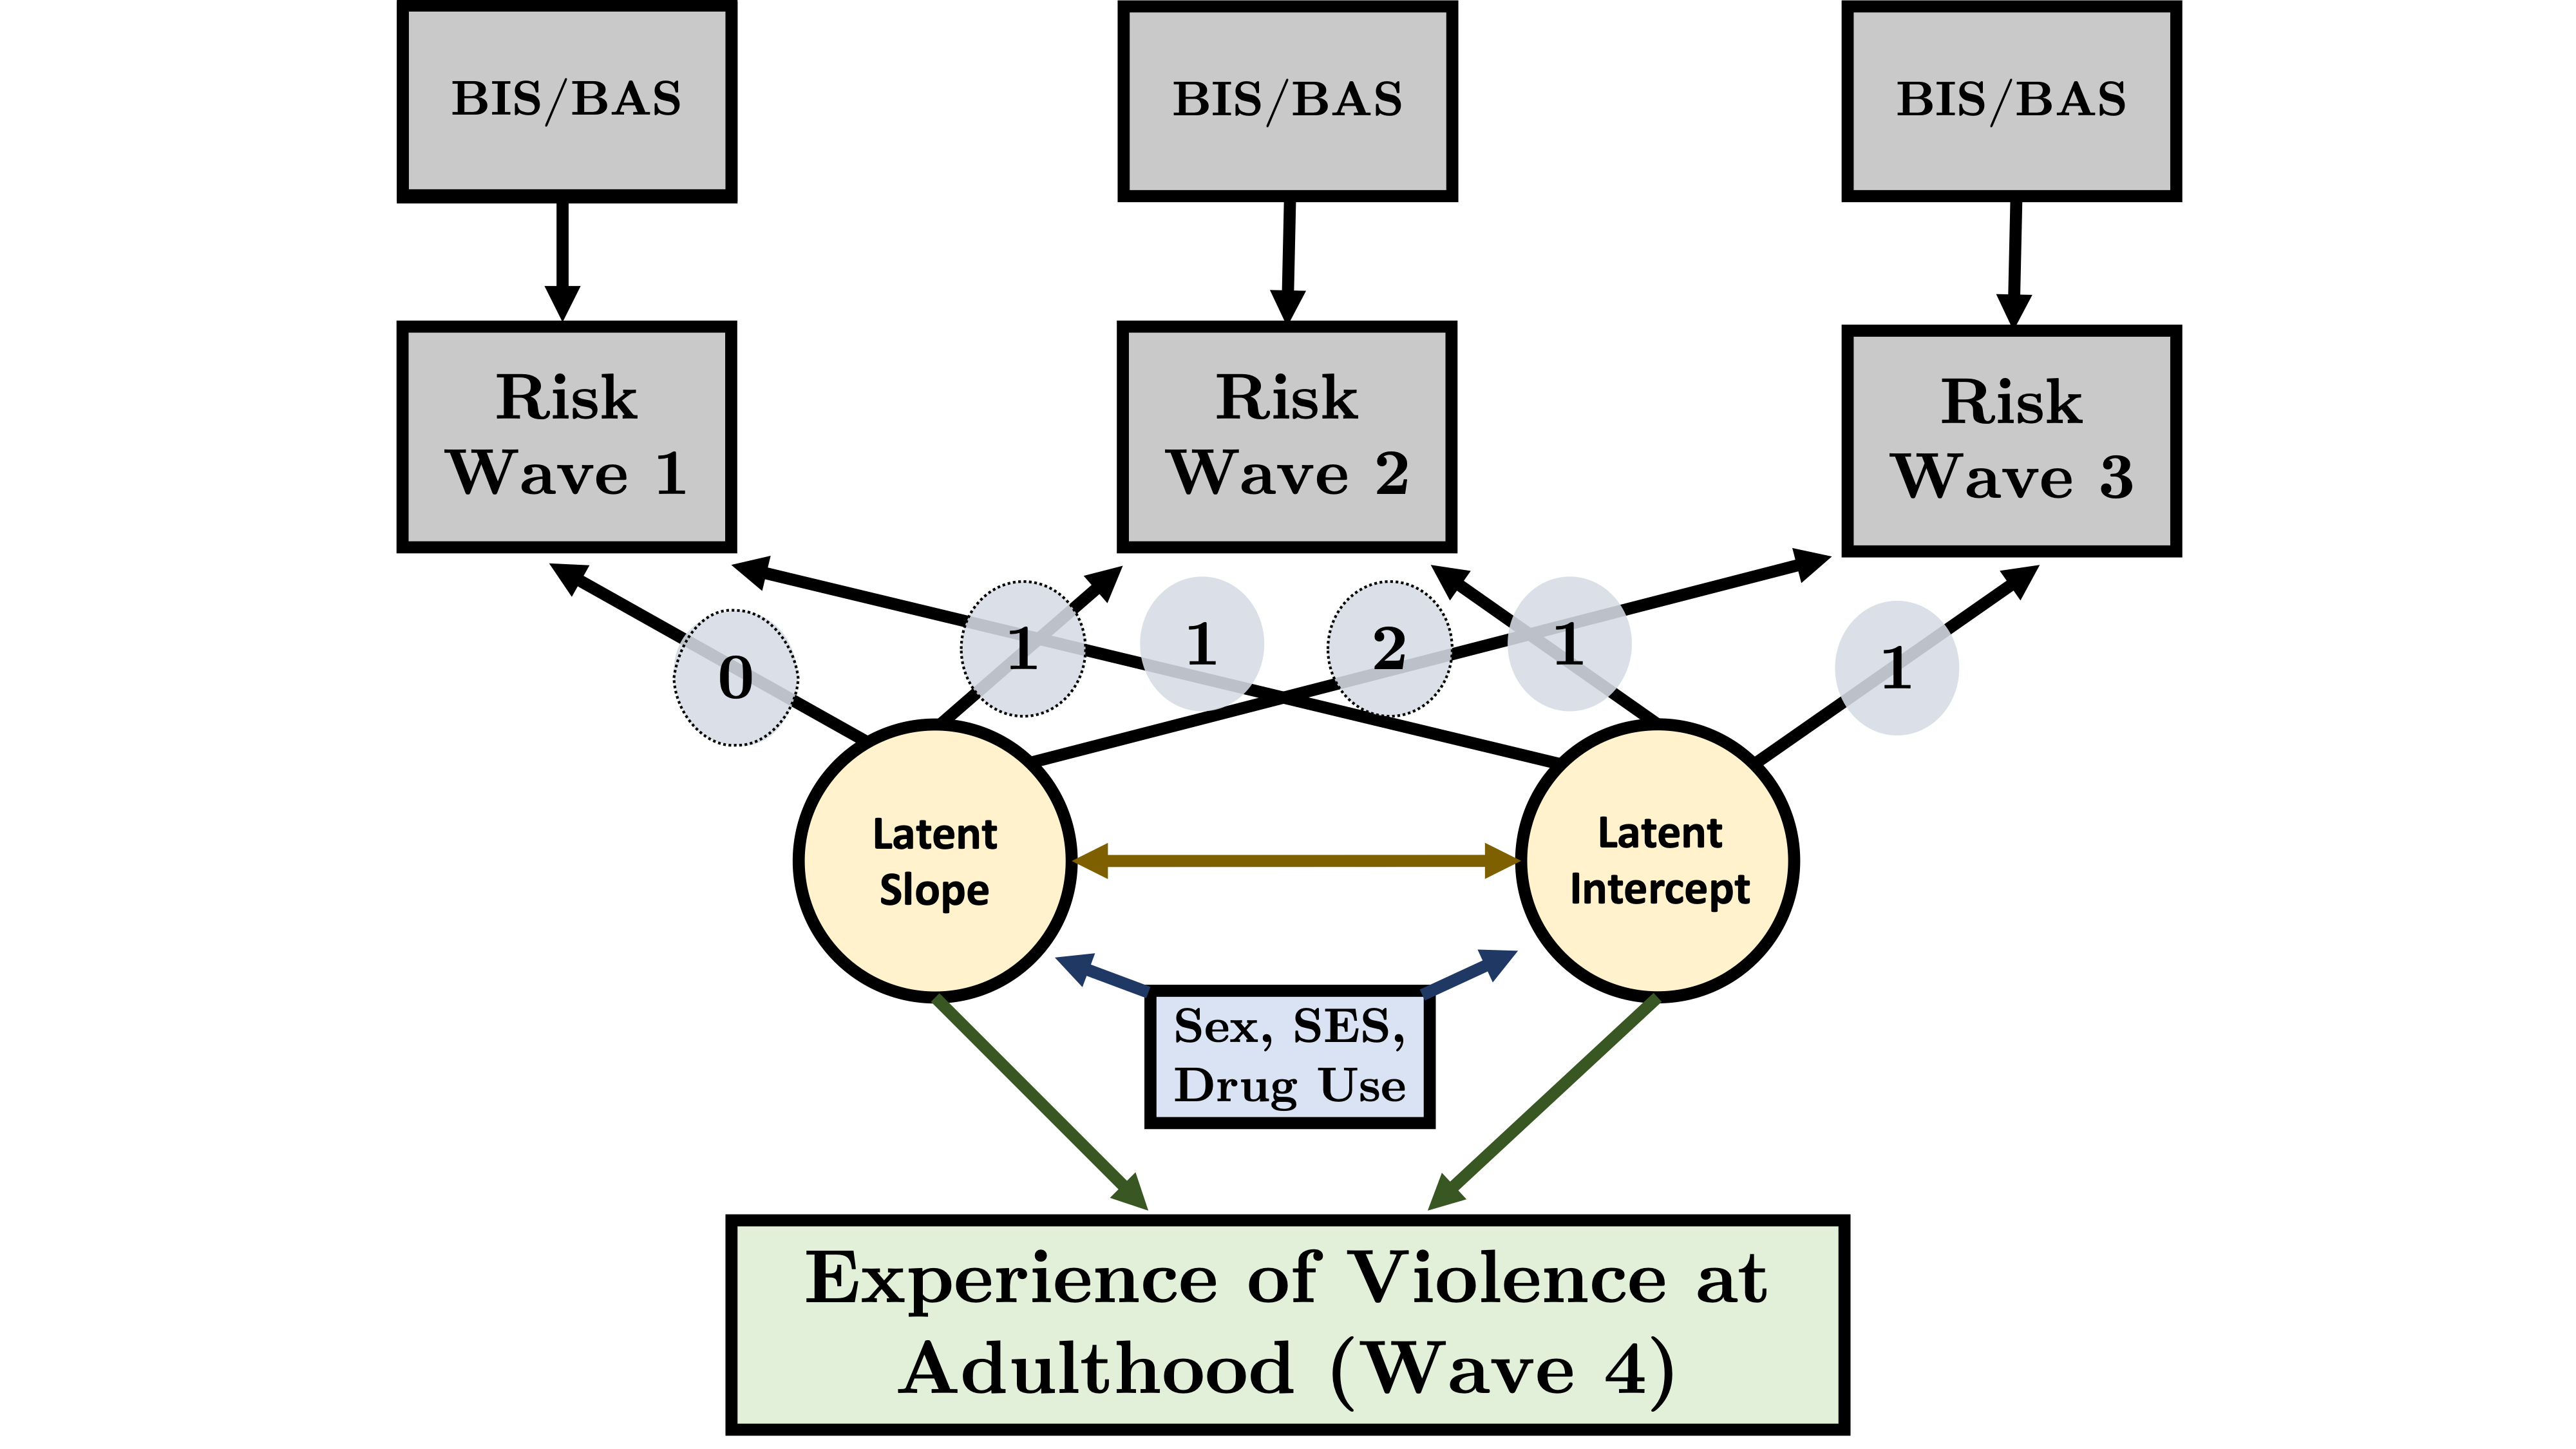
\includegraphics[width=\textwidth,height=\textheight,keepaspectratio]{Fig-1}
\caption{\textbf{Latent Growth Curve Model of Developmental Violence Risk.} A latent growth curve model was fitted to violence risk at each wave using the BIS/BAS scales as covariates. A linear latent slope factor was defined with 0 weighting at wave one, 1 weighting at wave two and 2 weighting at wave three, indicating that risk should change linearly with time. A latent intercept value was held constant at 1 for each wave. Sex, SES and Drug Use were tested as significant covariates of the estimate slope and intercept. Slope and intercept were found to predict future violence experiences measured at wave four. Estimated parameters and summary statistics of the fit appear in Table \ref{tab:1}. \label{fig:1}}
\end{figure}
%
\begin{figure}[h!]
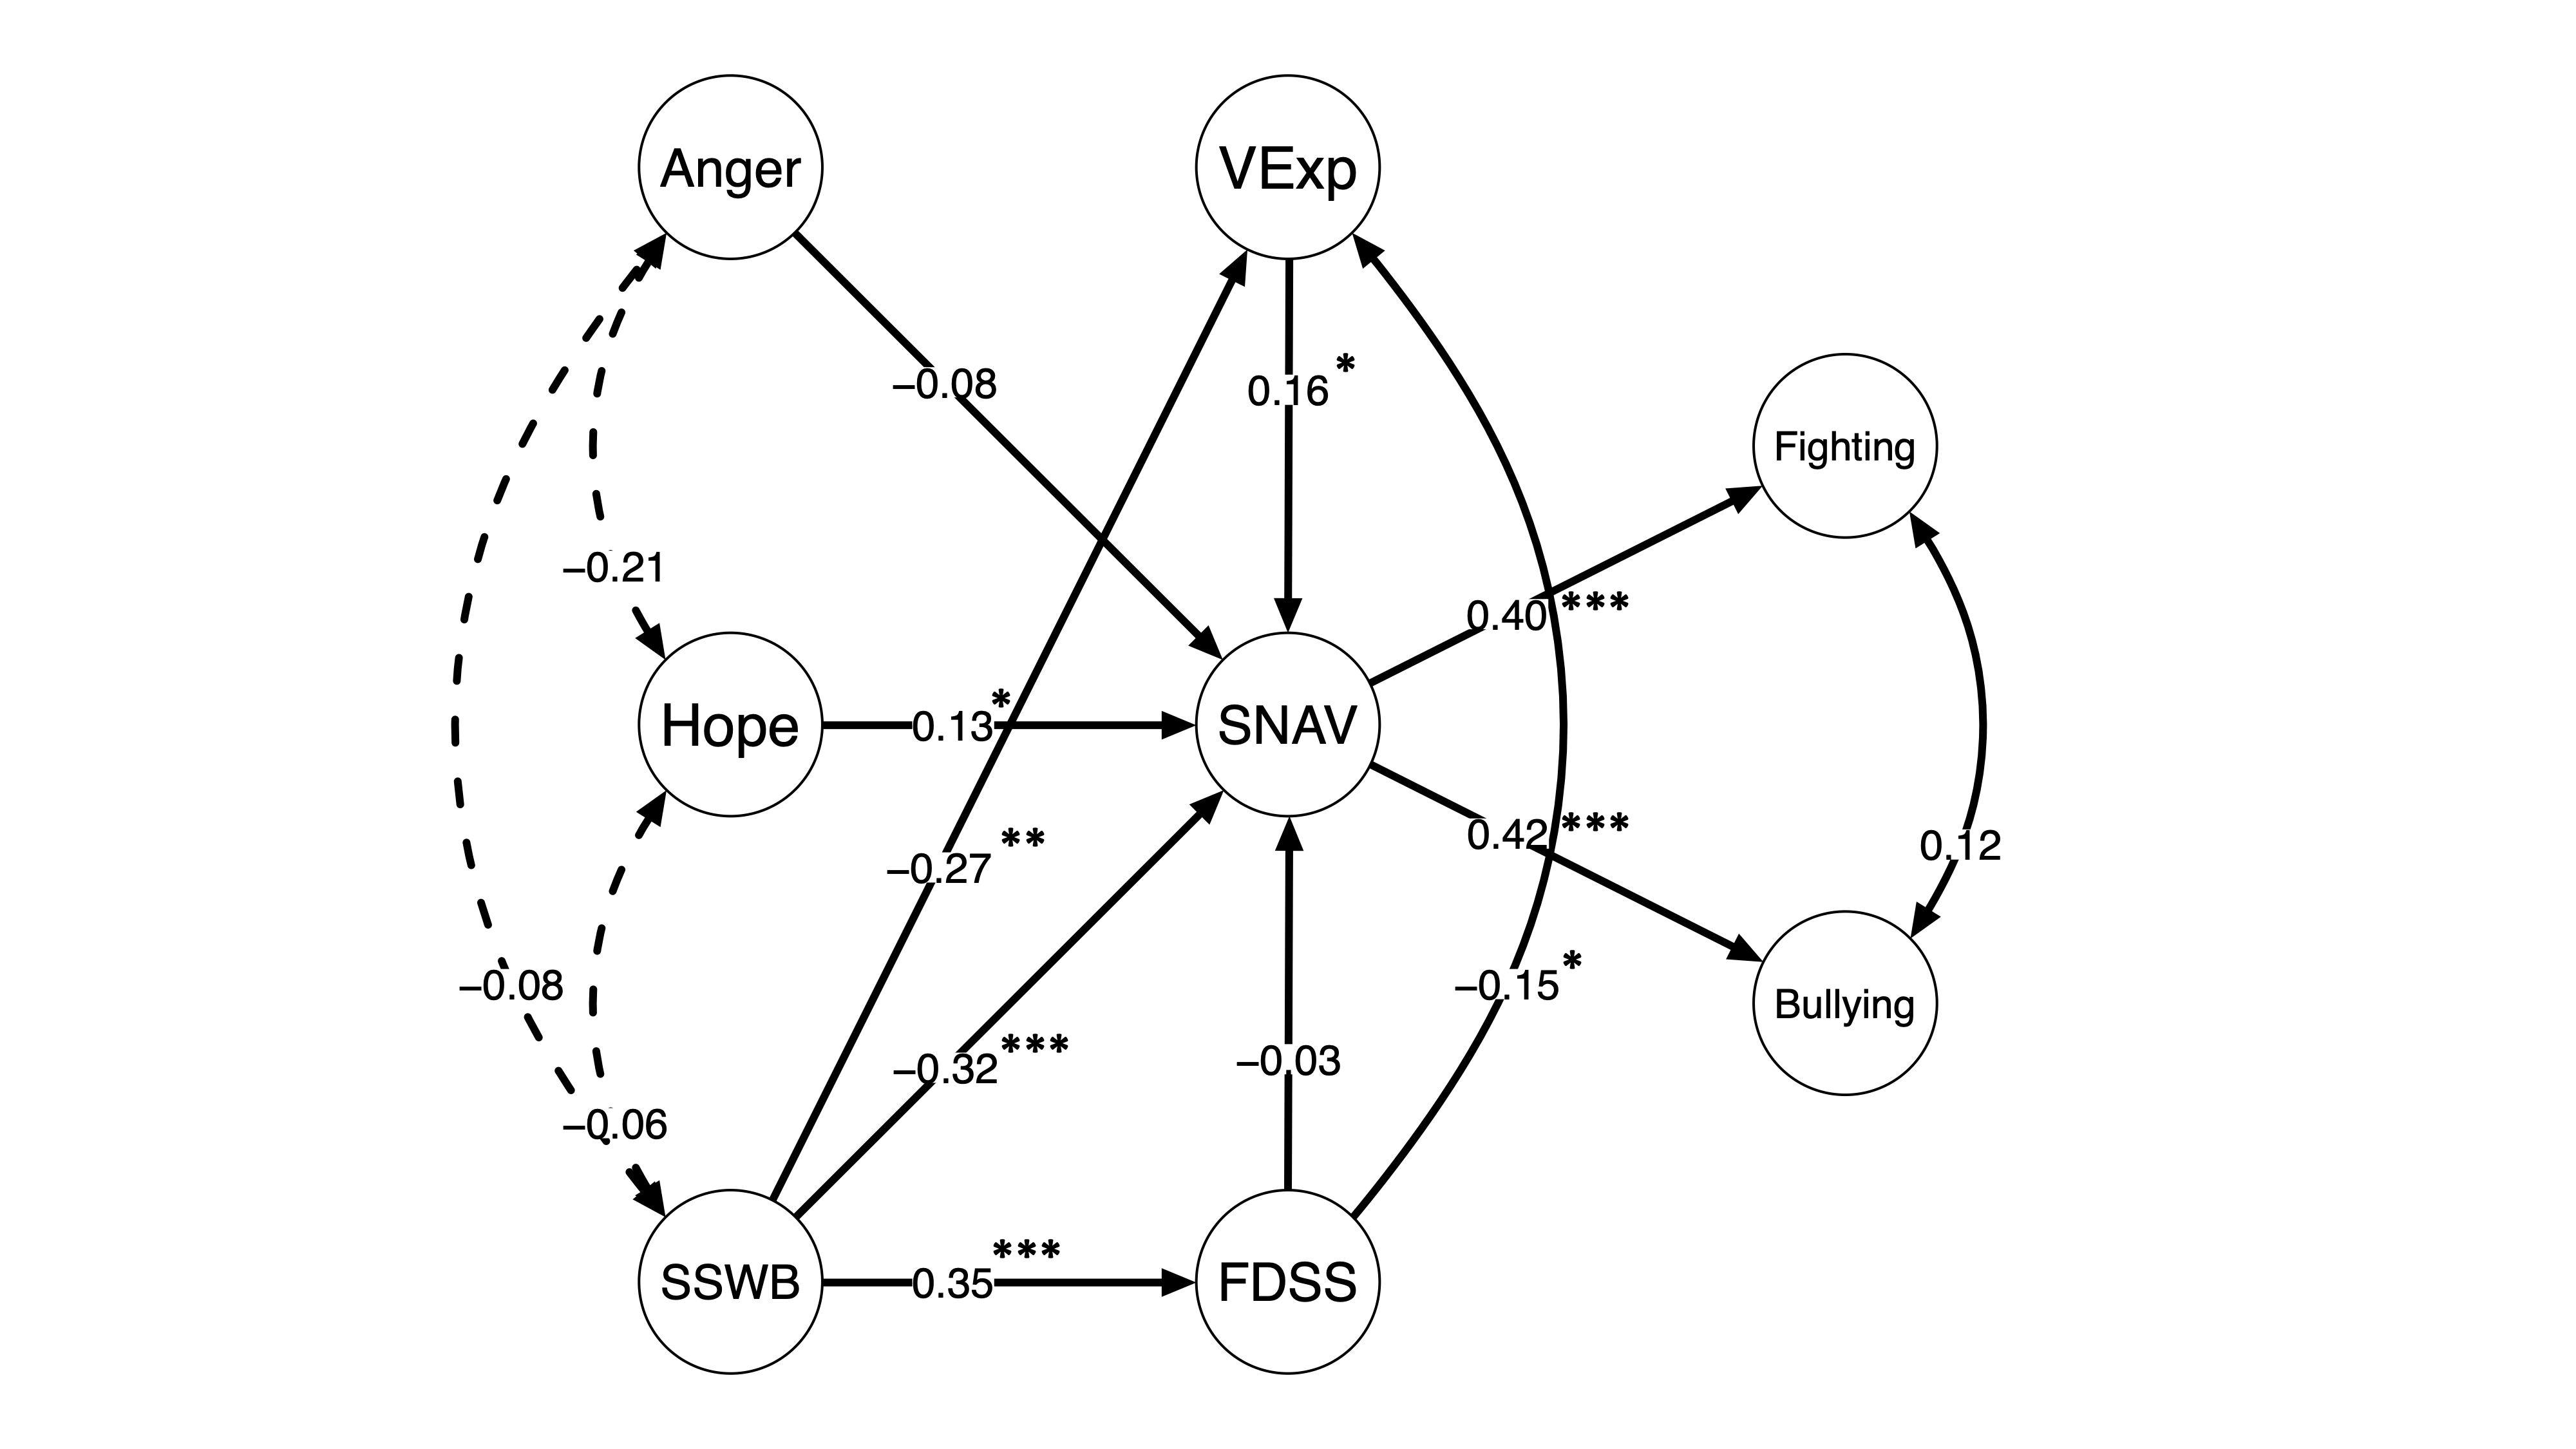
\includegraphics[width=\textwidth,height=\textheight,keepaspectratio]{Fig-2}
\caption{\textbf{Structural equation model of paths leading to altered social norms}. Social safety and well-being (SSWB) was hypothesized to directly and indirectly drive altered social norms by promoting healthy family dynamics and social support (FDSS), protecting against experiences of violence (VExp), and inhibiting the formation of proviolent attitudes (SNAV). All paths were significant from SSWB to SNAV except the direct path from FDSS and SNAV. Parameter estimates and summary statistics including the estimated coefficients for each mediation path are included in Tables \ref{tab:11} and \ref{tab:12}. \label{fig:2}}
\end{figure}

\clearpage
\section*{Tables}

%%%%%%%%%%%%%%%%%%%%%%%%%%%%%%%%%%%%%%%%%%%%%%%%%%%%%%
% Table :: DUSI-VP REGRESSIONS
%%%%%%%%%%%%%%%%%%%%%%%%%%%%%%%%%%%%%%%%%%%%%%%%%%%%%%
\begin{table}[h!]
\begin{tabular}{llllll}
DUSI-VP Latent Growth Curve Params                    & Estimate & Std. Error & Z-value & P($\textgreater{}\|z\|$) & Std. Estimate \\ \hline \\
\ \ \ Latent Intercept               & -0.073   & 0.117      & -0.620  & 0.535                    & -0.560  \\
\ \ \ Latent Slope                   & 0.178    & 0.068      & 2.608   & 0.009                    & 2.570  \\ \\
Regression on Latent Growth Curve Params  &          &            &         &                          &         \\ \hline \\ 
Latent Intercept               &          &            &         &                          &         \\
\ \ \ Sex                            & -0.012   & 0.031      & -0.374  & 0.708                    & -0.044  \\
\ \ \ SES                            & -0.064   & 0.018      & -3.543  & $\textless$0.001                    & -0.436  \\
\ \ \ Drug Use                         & 0.051    & 0.032      & 1.557   & 0.119                    & 0.190   \\
                               &          &            &         &                          &         \\
Latent Slope                   &          &            &         &                          &         \\
\ \ \ Sex                            & -0.019   & 0.020      & -0.963  & 0.336                    & -0.135  \\
\ \ \ SES                            & 0.028    & 0.012      & 2.362   & 0.018                    & 0.353   \\
\ \ \ Drug Use                         & 0.041    & 0.020      & 2.005   & 0.045                    & 0.289   \\
                               &          &            &         &                          &         \\
VExp                           &          &            &         &                          &         \\
\ \ \ Latent Intercept               & -0.112   & 0.142      & -0.789  & 0.430                    & -0.142  \\
\ \ \ Latent Slope                   & 0.343    & 0.170      & 2.025   & 0.043                    & 0.234   \\
\end{tabular}
\caption{\textbf{Latent growth curve model of developmental violence risk measured by DUSI-VP.} The Drug Use Screening Inventory risk of violence proneness (DUSI-VP) scores from waves one through three were used to fit intercept and slope parameters to a linear growth curve model of developmental violence risk. The latent slope estimate revealed a significant effect of change in risk across waves ($p=0.009$). The mean baseline risk did not significantly differ from zero across participants, although significant variation was observed. The effect of socioeconmic status (SES), sex and drug use at wave four were included as regression covariates of latent slope and intercept. Greater SES revealed lower baseline risk for violence ($p<0.001$) and elevated rate of risk accrual ($p=0.018$). The rate of risk accrual also predicted drug use in wave four ($p=0.045$). No significant effect found between baseline risk and sex or wave four drug use. Experiences of violence measured at wave four were found to be reliably predicted by latent slope ($p=0.043$) but not intercept. \label{tab:1}}
\end{table}
%%%%%%%%%%%%%%%%%%%%%%%%%%%%%%%%%%%%%%%%%%%%%%%%%%%%%%
% Table :: DUSI-VP REGRESSIONS
%%%%%%%%%%%%%%%%%%%%%%%%%%%%%%%%%%%%%%%%%%%%%%%%%%%%%%
\begin{table}[h!]
\begin{tabular}{llllll}
DUSI-VP Covariates                    & Estimate & Std. Error & Z-value & P($\textgreater{}\|z\|$) & Std. Estimate \\ \hline \\
                               &          &            &         &                          &         \\
DUSI-VP (Wave One)             &          &            &         &                          &         \\
\ \ \ BIS                            & 0.004    & 0.004      & 0.877   & 0.381                    & 0.072   \\
\ \ \ BAS-RR                         & 0.005    & 0.008      & 0.631   & 0.528                    & 0.054   \\
\ \ \ BAS-D                          & -0.000   & 0.007      & -0.033  & 0.974                    & -0.003  \\
\ \ \ BAS-FS                         & 0.011    & 0.007      & 1.525   & 0.127                    & 0.166   \\
                               &          &            &         &                          &         \\ \hline \\ 
DUSI-VP (Wave Two)             &     &     &   &                          &         \\
\ \ \ BIS                            & 0.009    & 0.005      & 1.841   & 0.066                    & 0.166   \\
\ \ \ BAS-RR                         & -0.012   & 0.009      & -1.228  & 0.219                    & -0.112  \\
\ \ \ BAS-D                          & 0.003    & 0.008      & 0.426   & 0.670                    & 0.043   \\
\ \ \ BAS-FS                         & 0.014    & 0.009      & 1.628   & 0.103                    & 0.170   \\ \\ \hline 
                               &          &            &         &                          &         \\
DUSI-VP (Wave Three)           &          &            &         &                          &         \\
\ \ \ BIS                            & -0.008   & 0.005      & -1.493  & 0.135                    & -0.141  \\
\ \ \ BAS-RR                         & 0.008    & 0.010      & 0.810   & 0.418                    & \ \ \ 0.075   \\
\ \ \ BAS-D                          & 0.000    & 0.010      & 0.015   & 0.988                    & 0.002   \\
\ \ \ BAS-FS                         & 0.003    & 0.010      & 0.281   & 0.779                    & 0.030   \\  
\end{tabular}
\caption{\textbf{BIS/BAS covariates of DUSI-VP latent growth curve model.} The behavioral inhibition system (BIS), behavioral approach, drive (BAS-D), behavioral approach, fun-seeking (BAS-FS), and behavioral approach, reward responsivity (BAS-RR) were included as covariates of DUSI-VP at each wave. No significant relationship was found comparing DUSI-VP to each of the BIS/BAS scales at each wave. \label{tab:2}}
\end{table}
%%%%%%%%%%%%%%%%%%%%%%%%%%%%%%%%%%%%%%%%%%%%%%%%%%%%%%
% Table :: VExp LATENT FACTOR
%%%%%%%%%%%%%%%%%%%%%%%%%%%%%%%%%%%%%%%%%%%%%%%%%%%%%%
\begin{table}[h!]
\begin{tabular}{lllll}
VExp Latent Factor & Estimate & Std. Error & Z-value & P($\textgreater{}\|z\|$) \\ \hline
                   &          &            &         &                          \\
VExp-P             & 0.066    & 0.025      & 2.627   & 0.009                    \\
VExp-O             & 0.019    & 0.009      & 2.076   & 0.038                    \\
VExp-V             & 0.104    & 0.021      & 4.955   & $\textless$0.001                    \\
VExp-PP            & 0.040    & 0.009      & 4.332   & $\textless$0.001                               
\end{tabular}
\caption{\textbf{Violence experience latent factor estimatation.} Cumulative violence experience (VExp) was estimated with confirmatory factor analysis using the perception (VExp-P), observation (VExp-O), victimization (VExp-V) and perpetration (VExp-PP) sub-scales of the Violence Experience Survey ($CFI = 0.99$, $TLI = 0.95$; $RMSEA = 0.028$, $p = 0.40$).  \label{tab:3}}
\end{table} 
%%%%%%%%%%%%%%%%%%%%%%%%%%%%%%%%%%%%%%%%%%%%%%%%%%%%%%
% Table :: VExp REGRESSIONS
%%%%%%%%%%%%%%%%%%%%%%%%%%%%%%%%%%%%%%%%%%%%%%%%%%%%%%
\begin{table}[h!]
\begin{tabular}{lllll}
VExp Covariates      & Estimate & Std. Error & Z-value & P($\textgreater{}\|z\|$) \\ \hline
                &          &            &         &                          \\
VExp           &          &            &         &                          \\
\ \ \ DUSI-VP         & 1.032    & 0.607      & 2.413   & 0.016                    \\
\ \ \ Sex             & -0.609   & 0.241      & -3.792  & $\textless$0.001                    \\
\ \ \ SES             & 0.007    & 0.102      & 0.069   & 0.945                    \\
\ \ \ BMI             & -0.047   & 0.043      & -1.106  & 0.269                    \\
\ \ \ IQ              & -0.006   & 0.008      & -0.748  & 0.455                    \\
\ \ \ BAS-D           & -0.011   & 0.031      & -0.358  & 0.720                    \\
\ \ \ BAS-FS          & -0.012   & 0.039      & -0.314  & 0.753                    \\
\ \ \ BAS-RR          & 0.057    & 0.042      & 1.373   & 0.170                    \\
\ \ \ BIS             & 0.028    & 0.022      & 1.283   & 0.200                    \\
                &          &            &         &                          \\ \hline \\ 
Drug Use          &          &            &         &                          \\ 
\ \ \ VExp            & 0.004    & 0.015      & 0.239   & 0.811                   
\end{tabular}
\caption{\textbf{Multivariate regression of violence experience.} Covariates of VExp were tested in a multivariate regression framework. Greater experiences of violence in adulthood were predicted by elevated violence risk in adolescence. Females reported greater experiences of violence than Males. No significant relationship between VExp and BIS/BAS sub-scales, SES, BMI or IQ was revealed. Violence experience did not predict elevated drug use in wave four. \label{tab:4}}
\end{table}
%%%%%%%%%%%%%%%%%%%%%%%%%%%%%%%%%%%%%%%%%%%%%%%%%%%%%%
% Table :: FDSS LATENT FACTOR
%%%%%%%%%%%%%%%%%%%%%%%%%%%%%%%%%%%%%%%%%%%%%%%%%%%%%%
\begin{table}[h!]
\begin{tabular}{lllll}
FDSS Latent Factor & Estimate & Std. Error & Z-value & P($\textgreater{}\|z\|$) \\ \hline
                   &          &            &         &                          \\
Fam-Co             & 0.091    & 0.011      & 7.940   & $\textless$0.001                    \\
Fam-Bf             & 0.041    & 0.009      & 4.846   & $\textless$0.001                    \\
Fam-St             & -0.179   & 0.014      & -12.912 & $\textless$0.001                    \\
Fam-Bd             & -0.103   & 0.019      & -5.287  & $\textless$0.001                    \\
Fam-Rx             & -0.175   & 0.020      & -8.677  & $\textless$0.001                    \\
Fam-Cf             & -0.075   & 0.011      & -6.608  & $\textless$0.001                    \\
SS                 & 0.058    & 0.017      & 3.461   & 0.001                   
\end{tabular}
\caption{\textbf{Family dynamics and social support latent factor estimation.} Normalized estimates for latent factors were estimated with confirmatory factor analysis to summarize family dynamics and social support (FDSS) measured with the Family Cohesion (Fam-Co), Positive Beliefs about Family (Fam-Bf), Family Disorganization \& Structure (Fam-St), Deviant Family Beliefs (Fam-Bd), Reactivity in Family Communication (Fam-Rx), Family Conflict (Fam-Cf), and the Vaux Social Support (SS) scales ($CFI=0.99$, $TLI=0.98$; $RMSEA=0.042$, $p=0.55$).\label{tab:5}}
\end{table}
%%%%%%%%%%%%%%%%%%%%%%%%%%%%%%%%%%%%%%%%%%%%%%%%%%%%%%
% Table :: FDSS REGRESSIONS
%%%%%%%%%%%%%%%%%%%%%%%%%%%%%%%%%%%%%%%%%%%%%%%%%%%%%%
\begin{table}[h!]
\begin{tabular}{lllll}
FDSS Covariates & Estimate & Std. Error & Z-value & P($\textgreater{}\|z\|$) \\ \hline
           &          &            &         &                          \\
FDSS       &          &            &         &                          \\
\ \ \ Sex        & 0.589    & 0.184      & 3.193   & 0.001                    \\
\ \ \ SES        & -0.190   & 0.108      & -1.754  & 0.079                    \\
\ \ \ BMI        & 0.013    & 0.024      & 0.544   & 0.587                    \\
\ \ \ IQ         & -0.007   & 0.005      & -1.337  & 0.181                    \\
\ \ \ DUSI-VP    & -1.735   & 0.518      & -3.351  & 0.001                    \\
\ \ \ BAS-D      & 0.059    & 0.037      & 1.579   & 0.114                    \\
\ \ \ BAS-FS     & -0.024   & 0.040      & -0.605  & 0.545                    \\
\ \ \ BAS-RR     & -0.098   & 0.046      & -2.121  & 0.034                    \\
\ \ \ BIS        & -0.005   & 0.022      & -0.220  & 0.826                    \\
           &          &            &         &                          \\ \hline \\
VExp       &          &            &         &                          \\
\ \ \ FDSS       & -0.220   & 0.067      & -3.265  & 0.001                   
\end{tabular}
\caption{\textbf{Multivariate regression of family dynamics and social support.} Covariates of FDSS were explored in a multivariate regression framework. Males reported greater FDSS compared to females ($p=0.001$). Greater average DUSI-VP in waves one through three was related to depressed FDSS in wave four ($p=0.001$). Elevated mean reward responsivity in waves one through three predicted lower FDSS in wave four ($p=0.034$). No significant relationship was found between FDSS and SES, BMI, IQ, BAS-D, BAS-FS or BIS. Greater family dynamics and social support was a protective factor against violence experience reported in wave four ($p=0.001$). \label{tab:6}}
\end{table}
%%%%%%%%%%%%%%%%%%%%%%%%%%%%%%%%%%%%%%%%%%%%%%%%%%%%%%
% Table :: SSWB LATENT FACTOR
%%%%%%%%%%%%%%%%%%%%%%%%%%%%%%%%%%%%%%%%%%%%%%%%%%%%%%
\begin{table}[h!]
\begin{tabular}{lllll}
SSWB Latent Factor & Estimate & Std. Error & Z-value & P($\textgreater{}\|z\|$) \\ \hline
                   &          &            &         &                          \\
NBR-C              & 0.187    & 0.040      & 4.731   & $\textless$0.001                    \\                   
NBR-R              & 0.018    & 0.019      & 0.917   & 0.359                    \\
NBR-D              & -0.031   & 0.019      & -1.596  & 0.111                    \\
NBR-CC             & -0.045   & 0.015      & -2.950  & 0.003                    \\
NBR-FC             & -0.021   & 0.017      & -1.222  & 0.222                    \\
SLE                & -0.065   & 0.010      & -6.160  & $\textless$0.001                   
\end{tabular}
\caption{\textbf{Social safety and well-being latent factor estimation.} Normalized estimates for latent factors were computed with confirmatory factor analysis to summarize Social Safety and Well-Being (SSWB) using measures of neighborhood cohesion (NBR-C), resources (NBR-R), disorganization (NBR-D), coping with community crime (NBR-CC),  fear of crime (NBR-FC), and stressful life events (SLE) measured at wave four ($CFI=0.98$, $TLI=0.92$; $RMSEA=0.071$, $p=0.26$).\label{tab:7}}
\end{table}


%%%%%%%%%%%%%%%%%%%%%%%%%%%%%%%%%%%%%%%%%%%%%%%%%%%%%%
% Table :: SSWB REGRESSIONS
%%%%%%%%%%%%%%%%%%%%%%%%%%%%%%%%%%%%%%%%%%%%%%%%%%%%%%
\begin{table}[]
\begin{tabular}{lllll}
SSWB Covariates  & Estimate & Std. Error & Z-value & P($\textgreater{}\|z\|$) \\ \hline
            &          &            &         &                          \\
SSWB        &          &            &         &                          \\
\ \ \ Sex         & 0.607    & 0.203      & 2.994   & 0.003                    \\
\ \ \ SES         & 0.054    & 0.195      & 0.275   & 0.784                    \\
\ \ \ BMI         & 0.093    & 0.030      & 3.064   & 0.002                    \\
\ \ \ IQ          & 0.010    & 0.008      & 1.304   & 0.192                    \\
\ \ \ DUSI-VP     & -2.664   & 0.607      & -4.388  & $\textless$0.001                    \\
\ \ \ BAS-D       & -0.056   & 0.055      & -1.030  & 0.303                    \\
\ \ \ BAS-FS      & -0.019   & 0.052      & -0.357  & 0.721                    \\
\ \ \ BAS-RR      & -0.005   & 0.061      & -0.081  & 0.935                    \\
\ \ \ BIS         & 0.013    & 0.034      & 0.375   & 0.707 \\ \\ \hline \\ 
VExp        &          &            &         &                          \\
\ \ \ SSWB        & -0.404   & 0.101      & -3.978  & $\textless$0.001                    \\
            &          &            &         &                          \\ \hline \\ 
Drug Use      &          &            &         &                          \\
\ \ \ SSWB        & -0.053   & 0.016      & -3.224  & $\textless$0.001                    \\
            &          &            &         &                          \\
\end{tabular}
\caption{\textbf{Multivariate regression of social safety and well-being.} Covariates of SSWB were explored in a multivariate regression framework. Females reported lower SSWB compared to males ($p=0.003$). Individuals with lower BMI also reported lower SSWB ($p=0.003$). Greater mean DUSI-VP measured from waves one through three predicted lower SSWB in wave four ($p<0.001$). No significant relation was found between SSWB and SES, IQ or the BIS/BAS scales. Elevated SSWB exhibited a protective effect on cumulative violence experience ($p<0.001$), whereas depressed SSWB predicted elevated drug use in wave four ($p<0.001$) \label{tab:8}}
\end{table}

%%%%%%%%%%%%%%%%%%%%%%%%%%%%%%%%%%%%%%%%%%%%%%%%%%%%%%
% Table :: SNAV LATENT FACTOR
%%%%%%%%%%%%%%%%%%%%%%%%%%%%%%%%%%%%%%%%%%%%%%%%%%%%%%
\begin{table}[]
\begin{tabular}{lllll}
SNAV Latent Factor & Estimate & Std. Error & Z-value & P($\textgreater{}\|z\|$) \\ \hline
                   &          &            &         &                          \\
AGV-S              & 0.196    & 0.032      & 6.136   & $\textless$0.001                    \\
AGV-A              & 0.340    & 0.054      & 6.329   & $\textless$0.001                    \\
AGV-E              & 0.235    & 0.036      & 6.484   & $\textless$0.001                    \\
AGV-P              & 0.263    & 0.050      & 5.207   & $\textless$0.001                    \\
AG                 & 0.019    & 0.010      & 1.892   & 0.059                    \\
PDV                & 0.014    & 0.013      & 1.041   & 0.298                    \\
ADQ                & -0.056   & 0.014      & -4.013  &$\textless$0.001                    \\
SR                 & -0.277   & 0.039      & -7.186  & $\textless$0.001                   
\end{tabular}
\caption{\textbf{Latent factor estimation of social norms and attitudes toward violence.} Normalized estimates for latent factors were obtained with confirmatory factor analysis to summarize Social Norms and Attitudes towards Violence (SNAV) calculated from the sub-scales of the Attitudes towards Guns and Violence which include: Shame (AGV-S), Excitement with Violence (AGV-E), Aggression (AGV-A) and Power for Safety (AGV-P). The Peer Deviancy (PDV), Aversion to Delinquency (ADQ), Attitudes toward Gangs (AG), and Social Responsibility (SR) are also included ($CFI=0.924$, $TLI=0.848$; $RMSEA=0.80$, $p=0.074$).\label{tab:9}}
\end{table}
%%%%%%%%%%%%%%%%%%%%%%%%%%%%%%%%%%%%%%%%%%%%%%%%%%%%%%
% Table :: SNAV REGRESSIONS
%%%%%%%%%%%%%%%%%%%%%%%%%%%%%%%%%%%%%%%%%%%%%%%%%%%%%%
\begin{table}[]
\begin{tabular}{lllll}
SNAV Covariates  & Estimate & Std. Error & Z-value & P($\textgreater{}\|z\|$) \\ \hline \\
SNAV                 &          &            &         &                          \\
\ \ \ Sex              & 0.593    & 0.202      & 2.942   & 0.003                    \\
\ \ \ SES              & -0.012   & 0.136      & -0.086  & 0.931                    \\
\ \ \ BMI              & -0.043   & 0.019      & -2.272  & 0.023                    \\
\ \ \ IQ               & -0.003   & 0.007      & -0.470  & 0.639                    \\
\ \ \ DUSI-VP          & 2.336    & 0.516      & 4.523   & $\textless$0.001                    \\
\ \ \ BAS-D            & 0.018    & 0.047      & 0.380   & 0.704                    \\
\ \ \ BAS-FS           & 0.066    & 0.045      & 1.489   & 0.137                    \\
\ \ \ BAS-RR           & -0.020   & 0.063      & -0.317  & 0.751                    \\
\ \ \ BIS              & -0.082   & 0.032      & -2.547  & 0.011                   \\
\ \ \ VExp             & 0.329    & 0.121      & 2.726   & 0.006                    \\
\ \ \ Drug Use           & 2.800    & 0.753      & 3.719   & $\textless$0.001                    
\end{tabular}
\caption{\textbf{Multivariate regression on social norms and attitudes toward violence.} Covariates of the SNAV latent factor were evaluated in a multivariate regression framework. Males reported greater antisocial and pro-violent attitudes compared to females ($p=0.003$). Lower BMI, lower average BIS, and greater average DUSI-VP was predictive of greater SNAV ($p=0.023$). Elevated violence experience and drug use in wave four was indicative of altered social norms ($p=0.006$). No significant relationship was found between SES, IQ, BAS scales and SNAV. \label{tab:10}}
\end{table}
%%%%%%%%%%%%%%%%%%%%%%%%%%%%%%%%%%%%%%%%%%%%%%%%%%%%%%
% Table :: SEM analysis
%%%%%%%%%%%%%%%%%%%%%%%%%%%%%%%%%%%%%%%%%%%%%%%%%%%%%%
\begin{table}[h!]
\begin{tabular}{llllll}
SEM Regressions &      & Estimate & Std. Error & Z-value & P($\textgreater{}\|z\|$) \\ \hline
                           &          &            &         &                          \\
FDSS                      &          &            &         &                          \\
& SSWB & 0.615   & 0.107      & 5.731  & $\textless$0.001 \\ \hline \\
SNAV                      &          &            &         &                          \\
& SSWB & -0.419   & 0.095      & -4.399  & $\textless$0.001 \\ 
& FDSS & -0.036   & 0.054      & -6.72  & 0.501 \\ 
& VEXP & 0.245   & 0.082      & 2.991  & 0.003 \\  \hline \\
VExp                      &          &            &         &                          \\
& FDSS & -0.097   & 0.044      & -2.232  & 0.026 \\ 
& SSWB & -0.299   & 0.076      & -3.938  & $\textless$0.001 \\ 
\end{tabular}
\caption{\textbf{Structural equation model of latent factor estimates.} Each latent factor estimate for family dynamics and social support (FDSS), social safety and well-being (SSWB), social norms and attitudes toward violence (SNAV), and cumulative experiences of violence (VExp) were input into a structural equation model. Paths to SNAV starting from SSWB and moving through FDSS and VExp were first tested with weighted parameter estimates of each pairwise regression. FDSS was directly driven by SSWB ($p<0.001$) and exhibited a protective effect on VExp ($p=0.026$). VExp was directly effected by SSWB ($p<0.001$) and was significantly related to variations in SNAV ($p<0.001$). SSWB directly drove SNAV ($p<0.001$). \label{tab:11}}
\end{table}

%%%%%%%%%%%%%%%%%%%%%%%%%%%%%%%%%%%%%%%%%%%%%%%%%%%%%%
% Table :: Path Analysis
%%%%%%%%%%%%%%%%%%%%%%%%%%%%%%%%%%%%%%%%%%%%%%%%%%%%%%
\begin{table}[h!]
\begin{tabular}{llllll}
Mediation Path Analysis &      & Estimate & Std. Error & Z-value & P($\textgreater{}\|z\|$) \\ \hline
                           &          &            &         &                          \\
Path $1$ :: VExp                       &          &            &         &                          \\
\ \ \ SSWB (direct) & -0.297   & 0.076      & -3.913  & $\textless$0.001                    \\
\ \ \ FDSS (indirect) & -0.060   & 0.029      & -2.078  & 0.038                    \\ \hline  Total Path $1$ Effect                    & -0.357   & 0.072      & -4.965  & $\textless$0.001                    \\
                           &          &            &         &                          \\
Path $2$ :: SNAV                       &          &            &         &                          \\
\ \ \ SSWB (direct) & -0.335   & 0.084      & -3.962  & $\textless$0.001                    \\ 
\ \ \ VExp (indirect) & -0.045   & 0.024      & -1.820  & 0.069                    \\
\ \ \ VExp (direct)  & 0.150    & 0.073      & 2.042   & 0.041                    \\
\ \ \ FDSS (indirect)  & -0.009   & 0.006      & -1.457  & 0.145                    \\ \hline
Total Path $2$ Effect                      & -0.379   & 0.082      & -4.604  & $\textless$0.001                    \\
                           &          &            &         &                          \\
Total Path $1+2$ Effect                     & -0.439   & 0.086      & -5.105  & $\textless$0.001                   
\end{tabular}
\caption{\textbf{Mediation analysis of paths to altered social norms.} Structural equation modeling was used to explore two complementary paths to altered social norms represented as elevated SNAV. Path $1$ showed a significant direct relationship from depressed social safety and well-being to elevated experiences of violence ($p<0.001$) and indirect path to VExp through fragmentation of family and social support ($p=0.038$). Path $2$ revealed elevated experiences of violence, mostly directly ($p=0.041$) and partially indirectly through depressed SSWB ($p=0.069$), caused greater acceptance of antisocial behavior. Family dynamics and social support did not exhibit a direct or indirect relationship with SNAV. Depressed SSWB was the strongest determinant of antisocial disposition ($p<0.001$). The total effect of both paths leading from SSWB through FDSS to VExp and from SSWB through VExp showed a significant total mediation ($p<0.001$). Table shows coefficient estimates of tested paths. \label{tab:12}}
\end{table}

%%%%%%%%%%%%%%%%%%%%%%%%%%%%%%%%%%%%%%%%%%%%%%%%%%%%%%
% Table :: PATH MODEL REGRESSIONS
%%%%%%%%%%%%%%%%%%%%%%%%%%%%%%%%%%%%%%%%%%%%%%%%%%%%%%
\begin{table}[]
\begin{tabular}{llllll}
SNAV Regression &       & Estimate & Std. Error & Z-value & P($\textgreater{}\|z\|$) \\ \hline
                      &       &          &            &         &                          \\
SNAV                  &       &          &            &         &                          \\
                      & H     & 0.803    & 0.362      & 2.217   & 0.027                    \\
                      & MAg-A & -0.360   & 0.353      & -1.019  & 0.308                    \\
                      &       &          &            &         &                          \\
MAg-B                 &       &          &            &         &                          \\
                      & SNAV  & 0.108    & 0.018      & 5.877   & $\textless$0.001                    \\
                      &       &          &            &         &                          \\
MAg-F                 &       &          &            &         &                          \\
                      & SNAV  & 0.060    & 0.010      & 6.122   & $\textless$0.001                   
\end{tabular}
\caption{\textbf{Normative social attitudes and perpetration of violence.} Antisocial and pro-violent attitudes were elevated with greater Hopelessness (H; $p=0.02$) but was not related to self-reported anger (MAg-A). Greater SNAV was related to elevated bullying (MAg-B) and fighting (MAg-F) behavior($p<0.001$). \label{tab:13}}
\end{table}
%%%%%%
\clearpage
\begin{table}[]
\resizebox{\textwidth}{!}{%
\begin{tabular}{ll}
\textbf{Violence Victimization Survey}                                                                                                                                                                                                           &                                                                                                                                                                                                       \\ \hline
                                                                                                                                                                                                                                                 &                                                                                                                                                                                                       \\
\textbf{Perception of Violence}                                                                                                                                                                                                                  &                                                                                                                                                                                                       \\
                                                                                                                                                                                                                                                 &                                                                                                                                                                                                       \\
\begin{tabular}[c]{@{}l@{}}1-4. Within the last year, how often you heard of the following situations happening \\ to others in your neighborhood?\end{tabular}                                                                                  & Others being attacked, threatened or robbed                                                                                                                                                           \\
                                                                                                                                                                                                                                                 &                                                                                                                                                                                                       \\
                                                                                                                                                                                                                                                 & People being badly beat up                                                                                                                                                                            \\
                                                                                                                                                                                                                                                 &                                                                                                                                                                                                       \\
                                                                                                                                                                                                                                                 & Individuals being seriously threatened                                                                                                                                                                \\
                                                                                                                                                                                                                                                 &                                                                                                                                                                                                       \\
                                                                                                                                                                                                                                                 & Individuals being verbally or emotionally abused                                                                                                                                                      \\
                                                                                                                                                                                                                                                 &                                                                                                                                                                                                       \\
\begin{tabular}[c]{@{}l@{}}5. Within the last year, how often have you heard of the situations in the previous \\ questions where a police officer or other civil authority figure was the aggressor?\end{tabular}                               &                                                                                                                                                                                                       \\
                                                                                                                                                                                                                                                 &                                                                                                                                                                                                       \\ \hline
                                                                                                                                                                                                                                                 &                                                                                                                                                                                                       \\
\textbf{Observation of Violence}                                                                                                                                                                                                                 &                                                                                                                                                                                                       \\
                                                                                                                                                                                                                                                 &                                                                                                                                                                                                       \\
\begin{tabular}[c]{@{}l@{}}6-9. Within the last year, how often have you seen the following situations happen \\ to others in your neighborhood?\end{tabular}                                                                                    & Others being attacked, threatened or robbed                                                                                                                                                           \\
                                                                                                                                                                                                                                                 &                                                                                                                                                                                                       \\
                                                                                                                                                                                                                                                 & People being badly beat up                                                                                                                                                                            \\
                                                                                                                                                                                                                                                 &                                                                                                                                                                                                       \\
                                                                                                                                                                                                                                                 & Individuals being seriously threatened                                                                                                                                                                \\
                                                                                                                                                                                                                                                 &                                                                                                                                                                                                       \\
                                                                                                                                                                                                                                                 & Individuals being verbally or emotionally abused                                                                                                                                                      \\
                                                                                                                                                                                                                                                 &                                                                                                                                                                                                       \\
\begin{tabular}[c]{@{}l@{}}10. Within the last year, how often have you seen the situations in the previous \\ questions where a police officer or other civil authority figure was the aggressor?\end{tabular}                                  &                                                                                                                                                                                                       \\
                                                                                                                                                                                                                                                 &                                                                                                                                                                                                       \\ \hline
                                                                                                                                                                                                                                                 &                                                                                                                                                                                                       \\
\textbf{Violence Victimization}                                                                                                                                                                                                                  &                                                                                                                                                                                                       \\
                                                                                                                                                                                                                                                 &                                                                                                                                                                                                       \\
\begin{tabular}[c]{@{}l@{}}11-14. Within the last year, how often have the following things happened to you? \\ This includes any situations that involved another student, teacher, family member \\ or someone in your community.\end{tabular} & \begin{tabular}[c]{@{}l@{}}Verbal or emotional abuse directed towards you; that is, being called \\ names or having things said to you that make you feel bad about your self or afraid.\end{tabular} \\
                                                                                                                                                                                                                                                 &                                                                                                                                                                                                       \\
                                                                                                                                                                                                                                                 & Serious threats that made you fear for the personal safety of yourself or others.                                                                                                                     \\
                                                                                                                                                                                                                                                 &                                                                                                                                                                                                       \\
                                                                                                                                                                                                                                                 & Getting caught up in a physical confrontation that may or may not have included weapons                                                                                                               \\
                                                                                                                                                                                                                                                 &                                                                                                                                                                                                       \\
                                                                                                                                                                                                                                                 & Received an injury in a physical confrontation.                                                                                                                                                       \\
                                                                                                                                                                                                                                                 &                                                                                                                                                                                                       \\
\begin{tabular}[c]{@{}l@{}}15. Within the last year, how often have the situations in the previous questions \\ happened to you when in contact with a police officer or other civil authority figure?\end{tabular}                              &                                                                                                                                                                                                       \\
                                                                                                                                                                                                                                                 &                                                                                                                                                                                                       \\ \hline
                                                                                                                                                                                                                                                 &                                                                                                                                                                                                       \\
\textbf{Perpetration of Violence}                                                                                                                                                                                                                &                                                                                                                                                                                                       \\
                                                                                                                                                                                                                                                 &                                                                                                                                                                                                       \\
\begin{tabular}[c]{@{}l@{}}16-21. Within the last year, how often have you done the following things to other \\ friends, family or community members?\end{tabular}                                                                              & Hit, kicked, pushed or shoved someone when you were angry                                                                                                                                             \\
                                                                                                                                                                                                                                                 &                                                                                                                                                                                                       \\
                                                                                                                                                                                                                                                 & Got into a fight after drinking or getting high                                                                                                                                                       \\
                                                                                                                                                                                                                                                 &                                                                                                                                                                                                       \\
                                                                                                                                                                                                                                                 & Threatened someone to get what you wanted                                                                                                                                                             \\
                                                                                                                                                                                                                                                 &                                                                                                                                                                                                       \\
                                                                                                                                                                                                                                                 & Engaged in a physical confrontation because it was fun                                                                                                                                                \\
                                                                                                                                                                                                                                                 &                                                                                                                                                                                                       \\
                                                                                                                                                                                                                                                 & Engaged in a physical confrontation even though you didn't want to                                                                                                                                    \\
                                                                                                                                                                                                                                                 &                                                                                                                                                                                                       \\
                                                                                                                                                                                                                                                 & Engaged in a physical confrontation to protect yourself, friends or family                                                                                                                           
\end{tabular}%
}
\end{table}
\clearpage
\bibliography{eldamaty_ncmi_2020a}

\bibliographystyle{apa}


\end{document}
